\documentclass[draftclsnofoot,10pt,onecolumn]{IEEEtran} %!PN

\usepackage[margin=0.5cm]{caption}
\usepackage{lipsum}

\usepackage{longtable}
\usepackage{graphicx}   
\usepackage[export]{adjustbox} 
\usepackage{epstopdf}

\usepackage{pdfpages}

\usepackage{caption}

\usepackage{amssymb}                                         
\usepackage{amsmath}                                         
\usepackage{amsthm}                                          

\usepackage{alltt}                                           
\usepackage{float}
\usepackage{color}

\usepackage{hyperref}
\usepackage{url}

\usepackage{array}

\usepackage{balance}
\usepackage[TABBOTCAP, tight]{subfigure}
\usepackage{enumitem}

\newcommand{\ignore}[2]{\hspace{0in}#2} %Used for inline comments
\newcommand{\tab}{\hspace*{2em}} %For tabbing

\renewcommand{\labelenumii}{\theenumii}
\renewcommand{\theenumii}{\theenumi.\arabic{enumii}.}

\usepackage{pstricks, pst-node}

\usepackage{geometry}
%\usepackage{graphicx}
\geometry{textheight=10in, textwidth=7.5in, margin=0.75in}

\usepackage{listings}

\definecolor{mygreen}{rgb}{0,0.6,0}
\definecolor{mygray}{rgb}{0.5,0.5,0.5}
\definecolor{mymauve}{rgb}{0.58,0,0.82}
\linespread{1}

\lstset{ %
  basicstyle=\ttfamily,            % the size of the fonts that are used for the code
  breakatwhitespace=false,         % sets if automatic breaks should only happen at whitespace
  breaklines=true,                 % sets automatic line breaking
  captionpos=b,                    % sets the caption-position to bottom
  commentstyle=\color{mygreen},    % comment style
  escapeinside={\%*}{*)},          % if you want to add LaTeX within your code
  extendedchars=true,              % lets you use non-ASCII characters; for 8-bits encodings only, does not work with UTF-8
  keepspaces=true,                 % keeps spaces in text, useful for keeping indentation of code (possibly needs columns=flexible)
  keywordstyle=\color{blue},       % keyword style
  %numbers=left,                    % where to put the line-numbers; possible values are (none, left, right)
  %numbersep=10pt,                  % how far the line-numbers are from the code
  %numberstyle=\tiny\color{mygray}, % the style that is used for the line-numbers
  rulecolor=\color{black},         % if not set, the frame-color may be changed on line-breaks within not-black text (e.g. comments (green here))
  showspaces=false,                % show spaces everywhere adding particular underscores; it overrides 'showstringspaces'
  showstringspaces=false,          % underline spaces within strings only
  showtabs=false,                  % show tabs within strings adding particular underscores
  stepnumber=1,                    % the step between two line-numbers. If it's 1, each line will be numbered
  stringstyle=\color{mymauve},     % string literal style
  tabsize=8,                       % sets default tabsize to 8 spaces
  %title=\lstname                  % show the filename of files included with \lstinputlisting; also try caption instead of title
}

\lstdefinelanguage{JavaScript}{
  morekeywords={var, function},
  morecomment=[s]{/*}{*/},%
  morecomment=[l]//,%
  morestring=[b]",%
  morestring=[b]'%
}

\usepackage{hyperref}

\def\BibTeX{{\rm B\kern-.05em{\sc i\kern-.025em b}\kern-.08em
    T\kern-.1667em\lower.7ex\hbox{E}\kern-.125emX}}
    
%\usepackage{floatrow}
\usepackage{lipsum}

    
\renewcommand{\lstlistingname}{Code Snippet:}


\begin{document}
% Hide page numbers
\pagenumbering{gobble}

%\title{Using the Style File IEEEtran.sty} 
\title{Tools for Supporting Community Growth in Open Source \\ {\large CS463: Final Report Spring 2016}}

\author{Bruntmyer J. Author, OSU, Goossens M. Author, OSU, Nguyen H. Author, OSU}

%\markboth{Tools for Supporting Community Growth in Open Source}
%{Murray and Balemi: Using the style file IEEEtran.sty} %!PN
%{Murray and Balemi: Using the Document Class IEEEtran.cls} %!PN


\maketitle
%\thispagestyle{plain}\pagestyle{plain}
\begin{abstract}
For the past six months our group has been working on a project that is creating tools that
gives users the ability to look for open source community leaders that are
hosting events. These tools will allow
users to have the opportunity to find these events in order to become a
contributor to an open source project. This is done in the form of a website that
will have features for finding certain events dealing with open source projects
so that it can be easily accessible by people with a passion for wanting to
contribute to projects. Throughout this document, we look at what this team has
accomplished for each of the requirements that have been laid out, discussing problems
that have halted our progression through the project, and how we changed our timeline.
Also included are important images of the user interface we have decided
to use, along with pieces of code that we have completed. By the end of this document, 
you will get a complete picture of how we
reached our version 1.0 release.
\end{abstract}

\newpage

\pagenumbering{arabic}

\section{INTRODUCTION TO THE PROJECT}

The Community Driven Development project is sponsored by the Apache Software Foundation under Ross Gardler, Director and President of the company. The project was designed and prototyped by Gardler before being proposed to the senior software project class for Oregon State University. Development for the project hopes to achieve more involvement in terms of helping building upon the Open Source Community and helping it grow and gain more traffic. The prototype was regularly used by Gardler and many of the faculty from Apache and is continued to gain interest to the public. The importance of development of the project will promote more growth and allow more tools for users in the community to find and locate more events and get more involved in open source community groups and projects. The students assigned to work on this project were Justin Bruntmyer, Megan Goossens, and Hai Nguyen. Each member took upon equal and separate roles for the project. No specific roles were assigned as each member took part in doing part of the work for every task. Ross Gardler provided the initial prototype while the project was improved and implemented with the requested features as the term progressed.

\newpage
\tableofcontents

\newpage

\section{REQUIREMENTS DOCUMENT}
\subsection{Introduction to the Problem}
Open source projects are known for the code that is developed from them however that is not what causes these projects to either 
live or die. Though it is true that an open source group can survive without a viable community in most cases there is a class of 
open source projects that lives or dies on the strength of its community such as the Apache Software Foundation projects. 
Existing tools are in place for tracking activity within online communities however these tools focus on identifying customers to 
the open source projects. The problem that is being focused on is that new tools need to be made to identify community leaders so 
that community builders know who to engage with.

\subsection{Project Description}

The goal of this project is to build connections, collaborations, and identifications between community members and leaders in 
open source projects. This entails contributing to Apache Software Foundation’s existing software platform to create tools 
that identify and support community leaders and members. Better tools will help identify potential community leaders which will 
then allow community builders to engage with and support those leaders. Over the course of the project, consistent updates check 
what tools were used as intended and which ones could be improved and expanded. Evaluation of the tools implemented is done in
order to measure its significance and effectiveness.

The solution to this problem should be able to identify community leaders to people with a desire to improve the strength of 
a community around a specific project. This solution includes being able to observe Apache Software Foundation community activity 
on publicly available information such as meetups.com in order to identify those potential community leaders. The solution is 
to provide enough information to community builders to contact and engage with the leaders so that they can begin their 
own contributions to the projects.

\subsection{Requirement}

The end goal of our project is to create a tool for identifying community leaders for others to see and given the chance to 
get involved with by having a web page that will let users go through and view all of this data in one location. This data will 
be gathered from an algorithm that reaches out to meetups.com and use key terms to find community leaders. As a stretch goal we 
would like to have this algorithm gain data from other social media sites such as Facebook and Twitter.

We will be starting with a prototype that has been implemented which means we will need to start by fixing what doesn't work and 
then adding key features that we believe the project needs. In a final delivery there will be a patched version of the prototype 
with tool fixes along with new features to improve usability. 

\newpage

\newcolumntype{C}[1]{>{\centering\let\newline\\\arraybackslash\hspace{0pt}}m{#1}}

\begin{center}
\begin{longtable}{ | C{1cm} | C{7cm}| C{6cm} | C{2cm} |} 
\hline
REQ\# & Requirement & Priority & Expected Completion \\ 
\hline
1 & Gain access to source code of the Community Developments page & HIGH & 11/30/2015\\
\hline
2 & Fix the "People" page where the list of community leaders are shown & HIGH & 01/11/2016
\\
\hline
3 & Tweet at a person listed i the database & LOW & 03/14/2016
\\
\hline
4 & Add user accounts to the application and track when a user has tweeted an event & MEDIUM & 02/15/2016
\\
\hline
5 & List tweets about events and/or people via the app & MEDIUM & 02/22/2016
\\
\hline
6 & List tweets about events and/or people from twitter, but not via the app & MEDIUM & 02/29/2016
\\
\hline
7 & Export a list of people with information & LOW & 03/07/2016
\\
\hline
8 & Improve hashtag searching of application for better results on relevant events & HIGH & 02/08/2016*
\\
\hline
9 & Alpha Release &  & 02/08/2016
\\
\hline
10 & Improve the visuals of the tool looks as a whole & HIGH & 02/01/2016
\\
\hline
11 & Beta Release &  & 03/14/2016
\\ 
\hline
12 & Implement a system of finding events nearby a location entered or within radius of the user & HIGH & 02/08/2016*
\\
\hline
13 & Add feature to generate a profile for community developers to have contacting information easily view-able & HIGH & 01/25/2016
\\
\hline
14 & 1.0 Release &  & 05/20/2016
\\
\hline
\end{longtable}
*We expect this task to be more difficult, so we will work on the task in parallel to other tasks during that time.
\end{center}

\subsection{Alpha/Beta/1.0 Releases}
We plan to release the Alpha version of the project during week 6 of winter term where we will have multiple fixes complete for the tools that are already implemented in to the project that we are starting with. This will mean that the Alpha version will be a major patch on what is created already in order to improve the functionality of the current implementation. We plan to release the Beta version of the project during finals week of winter term where we will implement new tools for community leaders to manage their posts along with some other useful tools. Here we plan to have almost all of the functionality ready. Lastly version 1.0 will be released on May 16, 2016 which is the Monday prior to the engineering expo. This version will be our final release and should be bug free in the implementation of our project.

\subsection{Specifications of Requirements}
\begin{enumerate}
\item Gain access to source code of the Community Developments page \\

\begin{enumerate}
\item Gain access to the source code for the prototype to begin working.
\item This will be given by client as we will be collaborating with him on testing the functionality of the prototype.\\
\end{enumerate}

\item Fix the “People” page where the list of community leaders are shown \\
\begin{enumerate}
\item Currently takes a large amount of time in order for the "people" page to load as it shows the current people who are 
identified as community leaders.
\item Figure out why the page takes such a long time to load. Could be too much data and the algorithm for pulling up this 
page needs to be changed. 
\item Need to debug the causes of crashes by some browsers. \\
\end{enumerate}

\item Tweet at a person listed in the database. \\
\begin{enumerate}
\item There will be a button that a user can select to send a tweet to a person directly.
\item This will be sending the user to the twitter API in order for them to construct and send a tweet. \\
\end{enumerate}

\item Add user accounts to the application and track when a user has tweeted an event \\
\begin{enumerate}
\item This is so they don't inadvertently do it twice
\item Track date of tweet, tweet text and tweet ID
\item This enables the prototype to branch out further than meetups.com
\item Allows user to see what tweets they have tweeted about \\
\end{enumerate}

\item List tweets about events and/or people via the application \\
\begin{enumerate}
\item This should work for the current user and others
\item Allows retweet or sending as new tweet based on existing one
\item Have a button that will list the tweets that were tweeted via the application. \\
\end{enumerate}

\item Export a list of people and email addresses \\
\begin{enumerate}
\item The emails corresponding with the people will be exported as well
\item Will be in JSON, CSV and test format for easy consumption in other applications \\
\end{enumerate}

\item Improve hashtag searching of application to improve finding relevant events \\
\begin{enumerate}
\item The searching algorithm is currently returning data from meetups.com with searching for tag "apache" however this is not working correctly as it is pulling information that has nothing to do with open source projects and is very random.
\item The searching algorithm will need to be fixed so that it find the correct tags from meetups.com and pull the accurate data.
\item The stretch goal here is the be able to use this algorithm on multiple social media networks. \\
\end{enumerate}

\item Alpha Release \\
\begin{enumerate}
\item Alpha to be released the 6th week of winter term.
\item This version will have some fixes for the improvement on algorithm, mark event action, mark group action, import members action, import meetups action, and the people action.
\item If not completely fixed/implanted the project will at least handle them by throwing a message to the user saying this tool is under construction. \\
\end{enumerate}

\item Improve the visuals of the tool looks as a whole \\
\begin{enumerate}
\item Make the user interface look sharper and more appealing
\item Have the events and people information that is displayed when a user decides to look into more details about a person or even be more appealing as well. \\
\end{enumerate}

\item Beta Release \\
\begin{enumerate}
\item The Beta of the project will be released on finals week of winter term.
\item In the Beta the fixes from the fist Alpha should all be fixed correctly, and all of the tools that we wanted to add should be implemented but not necessary working correctly, at least has some functionality. \\
\end{enumerate}

\item Implement system of improved sorting of finding events by nearby location within radius of the user \\
\begin{enumerate}
\item The program will be able to get the location from the user and based on this location the nearest community leader events will be shown to the user. \\
\end{enumerate}

\item Add feature to generate a profile for community developers to have contacting information easily viewable \\
\begin{enumerate}
\item Based on the data collected from meetups.com to identify the community leader not only will the events be posted but the community leader will have a section where the user can easily view the contact information pulled from meetups.com. A link with their name.
\item This is not a collaboration communication tool but just a way to view the contact information. \\
\end{enumerate}

\item 1.0 Release. \\
\begin{enumerate}
\item This will be the final release where all of our implementations should be working correctly with no bugs.
\item This will be released on May 16, 2016 which is the Monday prior to the Expo. \\
\end{enumerate}
\end{enumerate}

\subsection{Risk Assessment}
\begin{enumerate}
\item Miscommunication on can happen in between the Community Development team currently working on the project.
\item Security issues, unwanted changes to source code from unauthorized individuals
\item Algorithms created cause even slower computation time for certain aspects of the website
\item If certain implementation is added and is miscommunicated to a function that was not originally discussed
\item Pulling data from meetups could be corrupted
\item Code does not match with already implemented coding standards on the project
\end{enumerate}

\subsection{Stretch Goals}
\begin{enumerate}
\item Create a notification system to alert users of important events that the user may be interested in.
\item Create profile system for users and community developers
\item Create a notification system to alert users of important events that the user may be interested in
\item The project will have a tool that will allow a user to enter their email and they will be notified when a project event is added that they may be interested in.
\begin{enumerate}
\item This could also be implemented to send emails to users that sign up for them to a certain community leader for a certain project rather than trying to figure out what they might be interested in.
\end{enumerate}

\item Fix "Import Members” to allow importing of members
\item Allow community developers to edit their own events for specific messages
\item Create profile system for users and community developers
\end{enumerate}
\subsection{Time Table Gant Chart}
The gantt chart below shows the timeline we have set for our group to meet the requirements proposed in this document. We will be trying to fulfill this timeline as much as possible in a timely manner as it gives us a great path towards completing this project.

See gantt chart on next page.

\newpage

%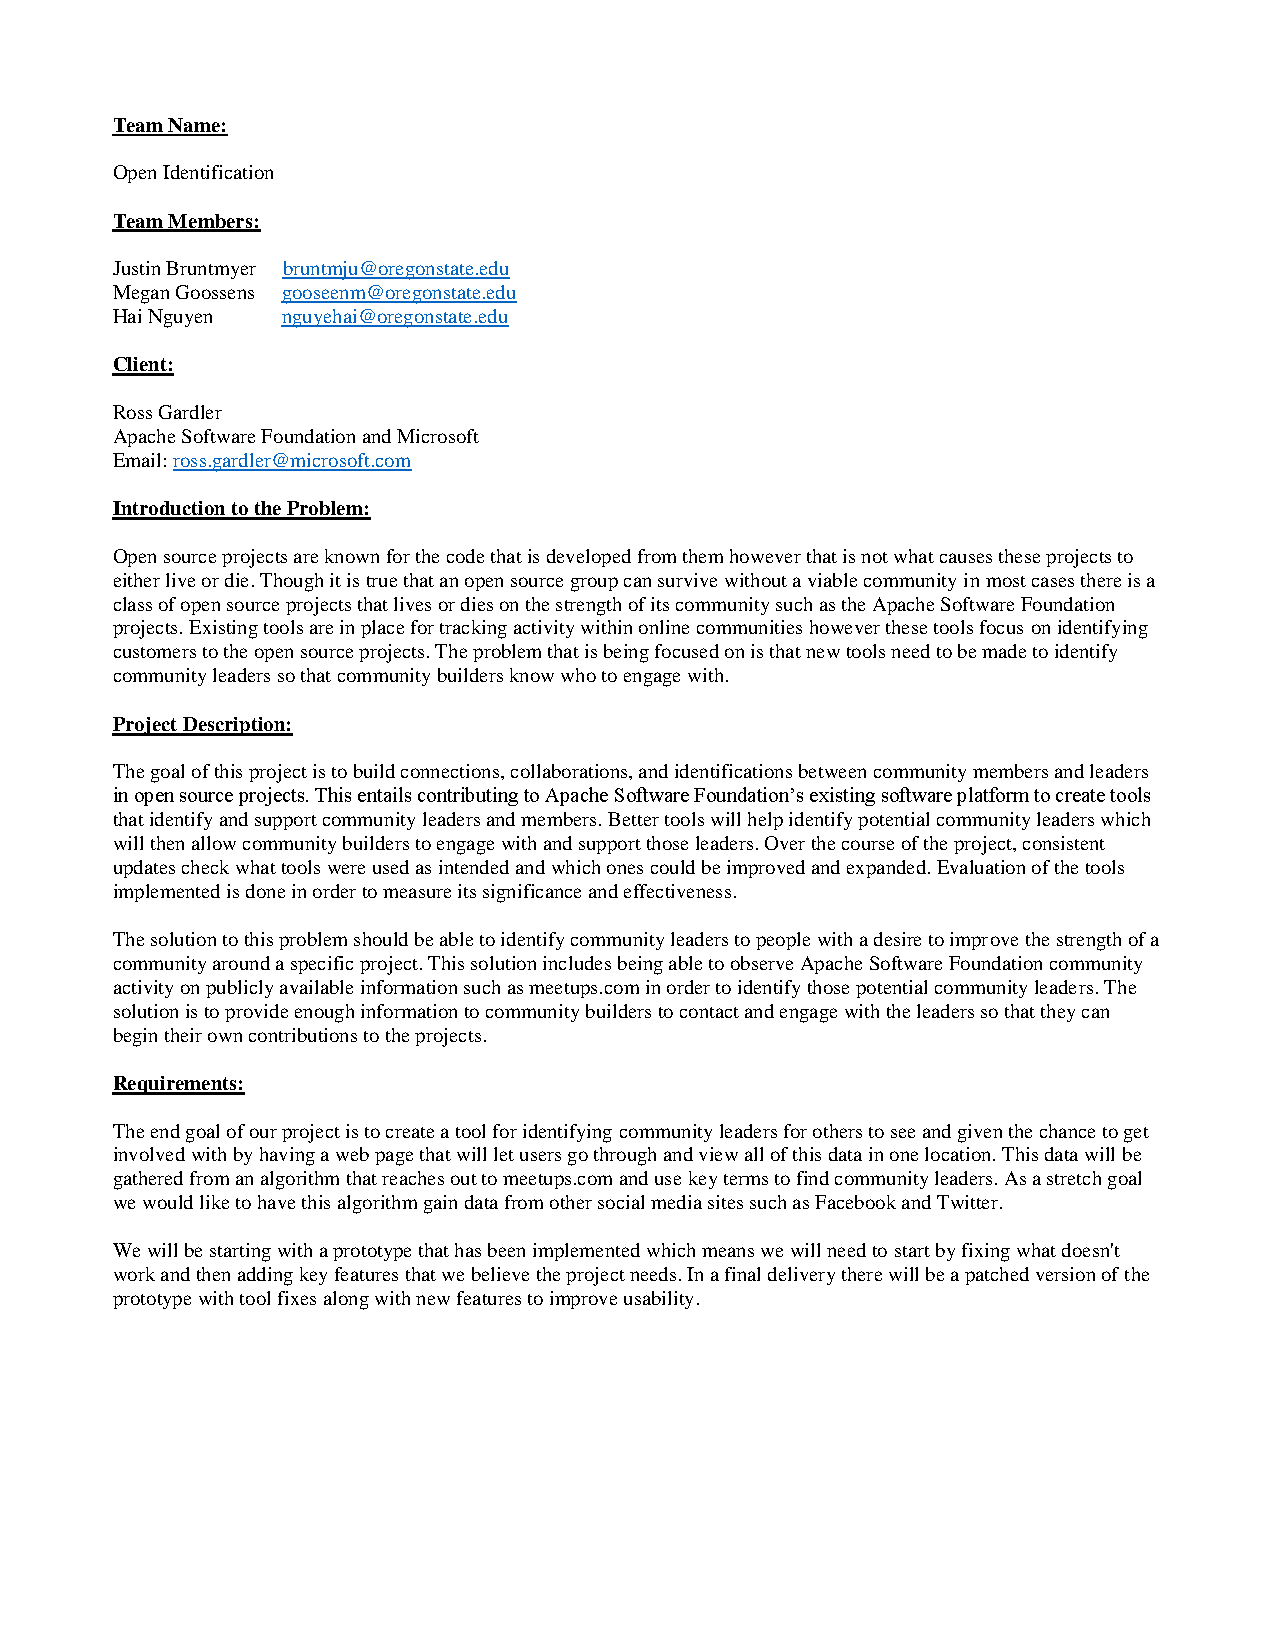
\includepdf[pages={-}, pagecommand={}]{Requirements_Document1.pdf}


\includepdf[pages={8, 9}, pagecommand={}]{Requirements_Document2.pdf}

\section{CHANGES TO THE REQUIREMENTS}
After continuous work on this project, the perspective on what
this community development tool wants to accomplish became clear. After taking
more time to read and understand the code that was previously written for the
prototype, we can see clearly how the data is organized and connected
using Django and its tools. First and foremost, the purpose of the community
development tool remains the same. The purpose is to gather information from
meetup.com which is the website we are pulling information about events and people from.
Next we parse that information into a list of upcoming events related to
Apache and open source projects so that developers in the open source community
have an easy way to access an environment where they can hope to participate in those
events. The ultimate goal of this project is to create a set of tools that eager developers
can use to find events, view community leader profiles, and get involved.\\

\newcolumntype{C}[1]{>{\centering\let\newline\\\arraybackslash\hspace{0pt}}m{#1}}

\begin{center}
\begin{longtable}{ | C{1cm} | C{7cm}| C{6cm} | C{2cm} |} 
\hline
REQ\# & Requirement & What Happened To It & Comments \\ 
\hline
1 & Fix the "People" page where the list of people are shown from groups & The
    “People” page currently takes all of the people in the database and lists them
    onto the page. Normally, if the prototype is hosted on a local machine and the
    database is relatively small, then the page loads fine in a minimal amount of
    time. The issue is nested in the actual hosted site by Apache where hundreds of
    thousands people are imported into the database daily and dramatically slowing
    down the loading time of the page.  With our current progression of the project,
    we have not made significant progress into improving the loading time of the
    page. We use our own local host to import a small amount of members at a time
    and that requirement is set to be worked on shortly for Beta implementation. The
    guideline for working towards accomplishing this requirement is to limit the
    amount of people loaded at a time onto the page. For Beta, we have rearranged
    where the table is generated for the people page in the function within
    views.py. This change specifically was introduced because a bug was found where
    when the table is generated, then if the amount of people were too many, then
    the table would crash and not build. With the rearrangement, now the table does
    not break through a large build and now tends to load faster. Unfortunately, the
    implementation of the fix for the People page is local. We have yet to test it
    on the host that Apache is using to run the prototype currently. We predict that
    the fix will work but it will need to be approved and patched into the live site
    for clarification. & blah\\ 
\hline
2 & Tweet at a person listed in database & Each person who is imported into the
    application is generated their own profile page based off of their Meetups ID.
    Information from Meetups about the person’s profile is also parsed in the
    community development tool. Those profiles include displaying the twitter handle
    of the person. This was done by changing the Meetup API request so that we could
    get the correct information and then store that information in our database.
    This can be seen in code snippet 1 located below with the URL shown along with
    the 'if' statements to locate the twitter handle. This allows the user to get in
    contact with the person in a profile. Above the twitter handle is a button that
    has the Twitter symbol which allows the user to click and send a tweet at the
    person via Hoot-suite. The hoot-suite app is given the twitter handle of the
    person the user wants to tweet at and the URL of the persons page on our
    application for reference. The user signs in to compose the tweet and sends it
    under their Twitter account. The code snippet 2 located below shows the HTML
    encoding of the button used to create the Hootsuite connection and shows the
    retrieval of the twitter handle form the database with 'person.service'. Not all
    users have a Twitter handle registered with Meetups thus the tweet button does
    not have any use. To handle this case the tweet at button only appears on
    profiles of imported people that have a registered Twitter handle. & blah\\ 
\hline
3 & Add user accounts to the application and track when a user has tweeted an
    event & The purpose of adding user accounts to the applications is to be able to
    track when users tweeting about events or people. With the completion of this
    requirement, the account creation is working along with being able to sign in
    successfully with a confirmation of signing in by displaying a welcome message
    along with the user's username. There is also a login and logout button located
    in the top right section of the website on all pages allowing the user to login
    or logout at anytime. Everything is also backended with features of the website
    only existing if the user has an authorized account. This means that action
    functions within the application which include importing meetups, importing
    members, marking events as not applicable, and marking groups as not applicable
    to be behind being signed in.  This means if you are not logged in with the
    authorized account, you can't perform these actions. Note that the accounts
    created are allowed access to these features, but do not have access to the
    administrative page that deals with the Django database. & blah\\ 
\hline
4 & List tweets about events and/or people via the app &  We were unable to
    track the precise tweets made from our application, but we have found an
    alternative that mostly works. As shown in the code snippet, the website makes a
    call to Twitter's search API, requesting all tweets that contain a certain
    hashtag as well as the hashtag \#Meetup. The hashtags are the same as the ones
    used to get events from meetup.com. Once it has the tweets, it uses the id from
    each one to make another call to Twitter's OEmbed API, which sends back HTML
    that is used in the page's template to present embedded tweets to users. This
    still pulls a few tweets that are unrelated, but bit of filtering would work.
    Unfortunately this would be difficult, and is outside the scope of our project.
    & blah\\ 
\hline
5 & List tweets about events and/or people from twitter, but not via the app &
    The website now has a tweet parser. As shown in the code snippet, it sends a
    call to Twitter's search API, requesting all tweets with a certain hashtag. The
    hashtags are the same as the ones used to get events from meetup.com. Once it
    has the tweets, it uses the id from each one to make another call to Twitter's
    OEmbed API, which sends back HTML that is used in the page's template to present
    embedded tweets to users.  The search results currently contain all instances of
    the hashtag requested, even when they are not relevant to any event, or even
    open source. The search needs refinement, however, this will be difficult, and
    is not within the scope of the project & blah\\ 
\hline
6 & Export a list of people with information & When taking on this requirement
    we quickly realized that the Meetup API would not provide email address for its
    users which was understandable. We then looked at what other information would
    be useful to extract about the people that were loaded into the database. This
    lead us to export information such as name, twitter handle, bio, Meetup ID, URL,
    country, state, and city. The export can be executed by clicking on the 'Export
    Info' button located in the top left of the people page and creates a file in a
    XLSX format which can be directly opened or saved. & blah\\ 
\hline
7 & Improve hashtag searching of application for better results on relevant
    events & The solution to this issue was to change one word in the call to the
    meetup.com API. In the API there are many different restrictions you can use to
    request events. Two of them come into play here: "text" and "topic." The text
    query searches through the content of the events, while the topic query looks at
    the topics related to the group. The original query was looking at text, which
    resulted in a lot of unrelated events. The query was fixed to use "topic," which
    has reduced unwanted events significantly. A thourough examination of events
    imported resulted in no unrelated events pulled in. & blah\\ 
\hline
8 & Implement a system of finding events nearby a location entered or within
    radius of the user & This tool creates a list of all events parsed through the
    application and displays a marker for each even onto the Google Map displayed to
    the right of the lists of events. A user can search for a specific event by
    looking through the list and then seeing where this is on the map. This feature
    also asks the web browser of the user for the geo-location of the user in order
    to place a special marker on the map showing where the user is in reference to
    the rest of the markers. The user can decide weather or not to accept giving the
    their location to the application. The map is generated through Google Maps by
    using the Google Map API calls. This map was implemented with a search bar
    allowing the user to search for a location and see what events are in that
    location. With each search the map jumps to the searched location and is given a
    200 mile radius circle to show what events are within 200 miles of the user. In
    order to get the markers of each event to show up on the map the latitude and
    longitude of each event needed to be stored and accessed by the map. This was
    done by a Meetups API call as shown in code snippet 3. Once the API call is made
    the json object is returned and parsed to obtain information on the event
    including name, longitude, and latitude. Once the information is stored it is
    accessed in the JavaScript for the Google Map which can be seen in code snippet
    4 below. This is done by looping though a list of events and gather the name,
    longitude, and latitudes in order for the markers to display. When a user hovers
    over a marker on the map the name of the event is shown.  When there are no
    events imported a message stating "No Events Available" is displayed. & blah\\ 
\hline
9 & Add feature to generate a profile for community developers to have
    contacting information easily visable & The main goal of the tool is to promote
    community development in the open source scene. What this feature tackles is a
    way to display important information about people that are already involved with
    projects to those who would like to get involved. This feature generates
    profiles for event hosts along with members of groups that have been imported by
    the user. These profiles consist of the of selected person, Twitter handle,
    location, link to Meetups profile, last activity date, group associated with,
    topics they are interested in, a biography, and a picture of themselves.  In
    order to gather the information for these we had to make another API call to
    Meetups. First, we had to adjust the current API call for importing events to
    also gather the ID of the event hosts.  Once this ID was obtained the next step
    is another API call gathering information on each event hosts while searching
    with the ID's gathered. Once this information was obtained the profiles for
    event hosts and imported group members could be displayed in their own sections
    of the application.  With users having the options to see group members and
    event hosts there are more opportunities for these users to get involved. &
    blah\\ 
\hline
10 & Improve the visuals of the tool and how it looks as a whole. & The
    application itself began as a fairly organized piece. The navigation bar
    implementation really helps the user keep track navigating between each page.
    When viewing the list of events, the events are listed in chronological order
    starting with the most recent. There is a search bar available for the user to
    type in for a certain event that they wish to view. There are other sorting
    mechanisms to view those events in another sorting order.  Our focus in this
    requirement were to mainly to improve how data is displayed. This specifically
    applies to to the event page and people profiles. Along with the addition of the
    Host objects, the generated host profiles would have a visual update as well.
    As displayed in Figure 9, the improvement of the profile page is shown with
    categories specifically labelled and displayed in concrete areas of the page. If
    the certain variable does not exist, then the user can clearly see where that
    detail would go on the page.  Topics are more clearly organized have are
    configured under a scrollable table as well.  Overall, this addition makes the
    people profile page much more organized and legible.  In addition to the updated
    people profile page, the event page is also upgraded in Figure 10. Similar to
    the profile upgrade, the event page now has categories that specifically detail
    where objects belong. This is much more particularly important where the
    description is displayed for the event. Previously, it was much more difficult
    for the user's eye to view where the venue of event would be. Now in this
    update, that portion is clearly labelled which allows the user to spend less
    time reading and to quickly see the information that they want to. & blah\\ 
\hline
\end{longtable}
\end{center}

\newpage
%The design document is inserted here.
\section{DESIGN DOCUMENT}

%\begin{enumerate}
\subsection{Frontpiece}
	\begin{enumerate}
	
		\item Date of Issue and Status \\
		The design of the project was issued on October 4 th , 2015. The status of the project was already in production with a
		prototype.\\
		
		\item Issuing Organization \\
		The Apache Software Foundation originally began development of the project and issued the proposal to Oregon
		State University for continued development. This entails to contributing to Apache Software Foundation’s existing
		software platform to create tools that identify and support community leaders and members.\\
		
		\item Authorship \\
		Current developers contributing to the community tool include Ross Gardler, Justin Bruntmyer, Hai Nguyen, and
		Megan Goossens. Ross Gardler, president of Apache, is the original developer for the project.\\
		
		\item Change History \\
		
	\end{enumerate}
	
\subsection{Introduction}
	\begin{enumerate}
	
		\item Purpose \\
		The primary purpose of this document is to present a detailed description of the design elements of the Getting
		Connected: Tools for the Open Source Community project. This will guide the group in the design of the
		application.\\
		
		\item Scope \\
		This document will provide details on the design of the various technologies of the web application, in particular the
		Django framework, PostgreSQL, HTML user interface, and the user and group authentication system provided by Django.\\

		The user will have the ability to view the community leaders that are posting events on social media sites based on
		tags fetched by the tools. This will allow the user to see the activity and contact information of the community leader
		to potentially contact if the user is interested in contributing. The user will be able to view a summary of the event as
		well as have a link to the source of the event hosted by the community leader.\\
		
		\item Context \\
		This project will be free to access for everyone. Development and maintenance will have not cost as this project is
		open source. Future development plans will be based on the features that do not make it in the 1.0 release of the
		application. There are several stretch goals that will potentially be incorporated. These features are not covered in
		this document.\\
		
		\item Summary \\
		This document will go over the design for the aspects of the project including web framework, database design, user
		interface, and authentication system. \\
	\end{enumerate}

\subsection{References}
	\begin{enumerate}
	
		\item IEEE Standard for Information Technology--Systems Design--Software Design Descriptions, 1st ed. IEEE, 2009. \\
		
		\item Comdev1-us-west.apache.org, 'Community Development: Events', 2015. [Online]. Available: \\ http://comdev1-us-
		west.apache.org/events/. [Accessed: 03- Dec- 2015]. \\
		
		\item Djangoproject.com, 'The Web framework for perfectionists with deadlines | Django', 2015. [Online]. Available:
		https://www.djangoproject.com/. [Accessed: 03- Dec- 2015]. \\
		
		\item W3.org, 'HTML5', 2015. [Online]. Available: http://www.w3.org/TR/html/. [Accessed: 03- Dec- 2015]. \\
		
		\item Postgresql.org, 'PostgreSQL: The world's most advanced open source database', 2015. [Online]. Available:\\
		http://www.postgresql.org/. [Accessed: 03- Dec- 2015]. \\
		
	\end{enumerate}

\subsection{Glossary}

\begin{longtable}[1]{ | C{7cm} | C{7cm} |} 
\hline
Term & Definition \\ 
\hline
API & Application Programming Interface\\
\hline
Query & Request sent to a database
\\
\hline
Query Parameter & Argument sent to a database to refine a search
\\
\hline
Community Leader & Someone who is in charge of a project or organization
\\
\hline
Tags &  Keywords - e.g. "apache," "open source," etc.
\\
\hline
HTML & HyperText Markup Language
\\
\hline
Django & Web framework
\\
\hline
PostgreSQL & Database management system
\\
\hline
Meetup & Meetup.com
\\
\hline
\end{longtable}

\subsection{Body}
	\begin{enumerate}
		\item Identified Stakeholders and Design Concerns \\
		For the stakeholders, the tools support and help the Apache Software Foundation. Specifically, Ross Gardler is the
		main stakeholder that is part of the design.\\
		
		Concerns regarding the design of the project include completions of certain implementations with the requirements
		listed. Troubleshooting problems or possible encounters that may appear during implementation are listed as such.\\
		
		\item Algorithm Viewpoint \\
			\begin{enumerate}
				\item Fix the "People" page where profiles are not implemented \\
				As a high priority, fixing any type of design bug that was already implemented in the prototype is
				important. The page listed currently takes a very long time as a link from extracting all data from the
				PostgreSQL database causes difficulty in the time frame. Possible ways to approach in this solution
				include:
				\begin{itemize}
					\item Taking a look at how the data is sorted
					\item Looking at the users list and what is included in "People"
					\item Changing the algorithm in the time frame to extract the data.\\
				\end{itemize}
				
				\item Design View \\%pictuee goes here!!!!!!!!!!!!!!!!!!!!!!!!!!!!!!!!!!!!!!!!!!!!!!!!!!!!!!!!!!!!!! \\
				Our fixing the people page viewpoint shows how the application will be interacting with the Django
				framework along with the database. We know that the button on the webpage will be an HTML button that
				will be selected by the user. Once selected the Django framework will be activated to query the database
				for the current list of community leaders. Once the database finishes the query it will send the list back to
				the HTML page to be displayed for the user.\\
				
				\begin{figure}[H]
  					\begin{center}
						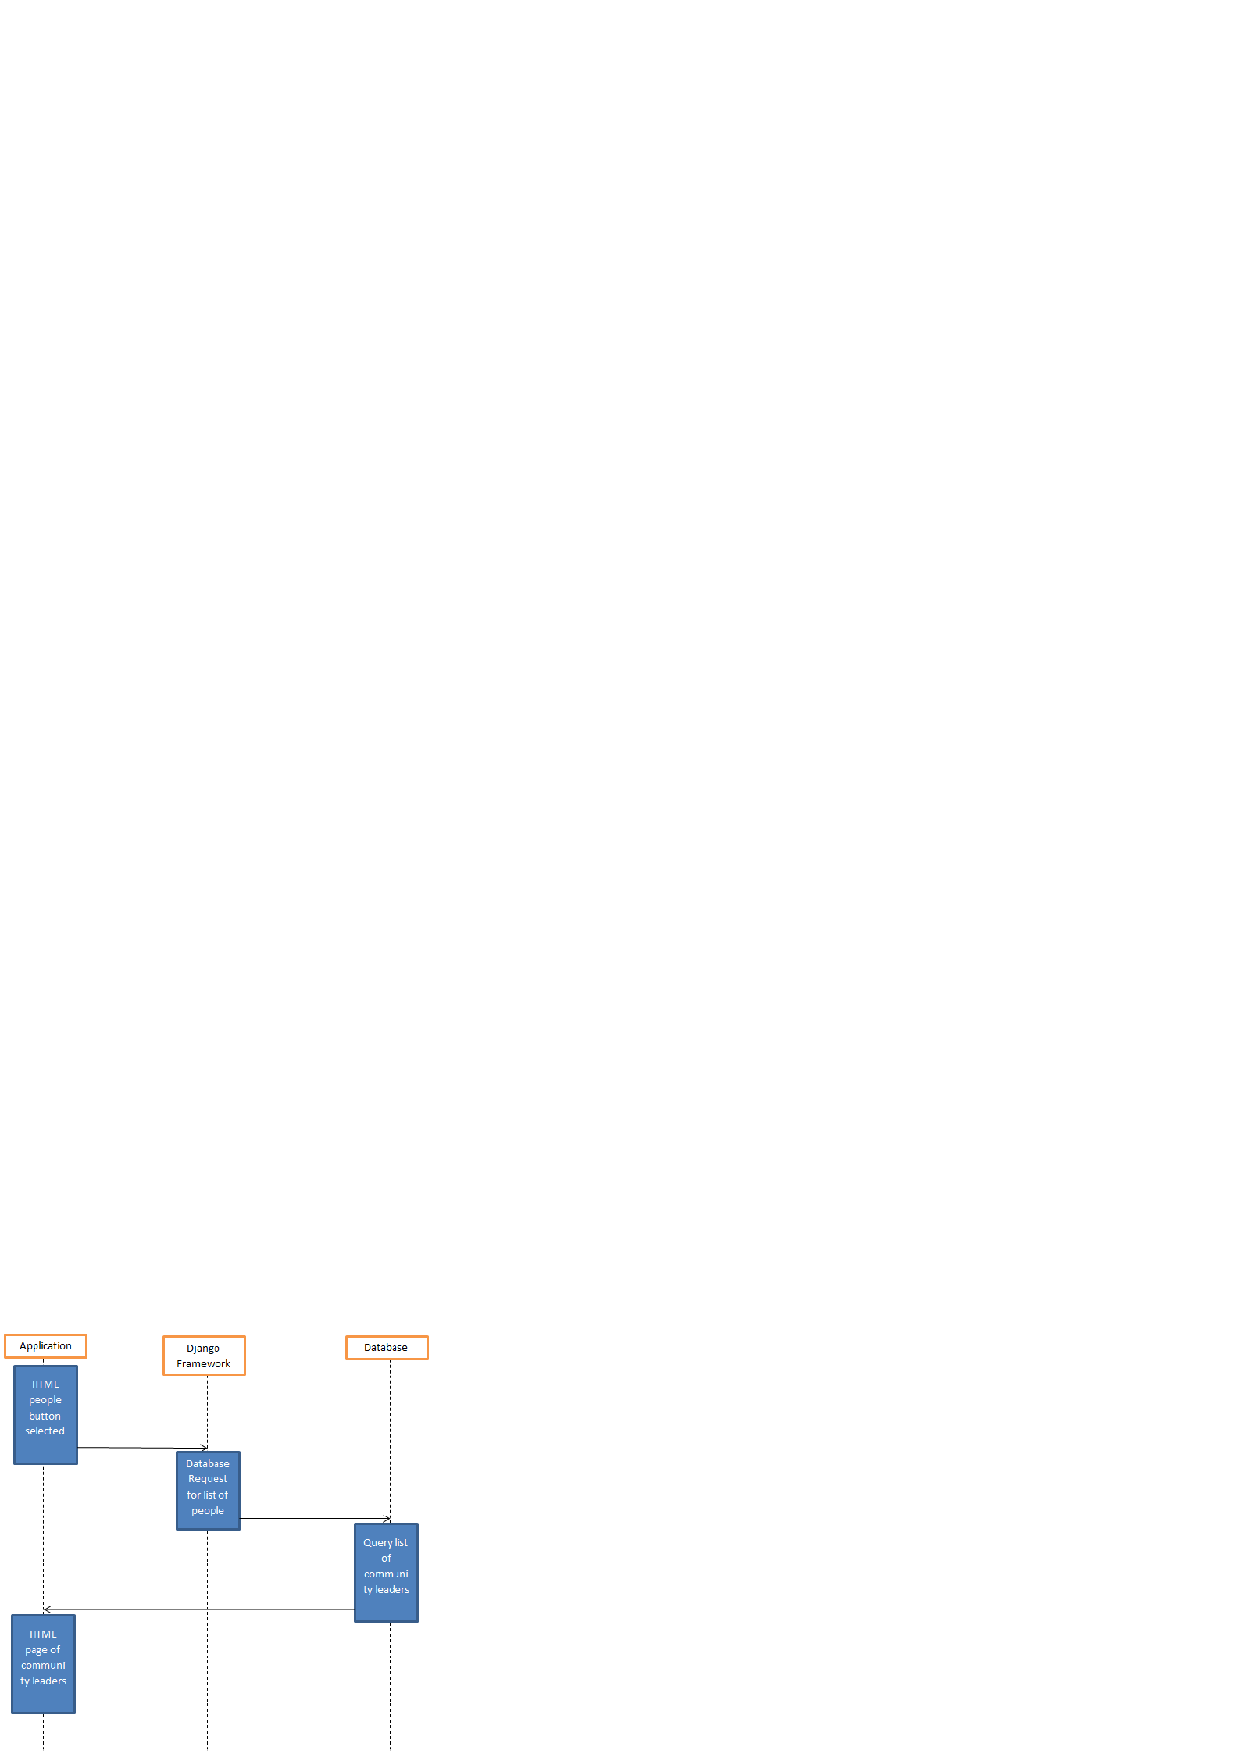
\includegraphics[width=4in, frame]{DD_1}
						\captionsetup{width=.4\linewidth}
						\centering
  						\caption{Sequence diagram of how the application will interact with the database and display the 
  						people page.}
  					\end{center}
				\end{figure}
				
				\item Design Rationale \\
				A look at how the various steps for loading the people page is necessary due to the fact that it is not
				obvious as to why the page is not loading properly. As there are several possible sources for the slowness,
				all of them must be examined to be able to determine the cause or causes. Once the problem has been
				pinpointed, the next step is to work on optimizing it, whether that involves changing how the data is stored,
				changing the query that fetches the data, or changing the algorithm that processes and presents the fetched
				data.\\
				
				\item Improve searching algorithm of tool for more relevant events\\
				The way the events are listed and how relevant they are to the user is important. With the prototype, events
				currently being extracted have the ability to not even be related to open source or programming itself.
				Implementing a new searching algorithm will be difficult and could cause a lot of troubleshooting listed
				below:
				\begin{itemize}
					\item Improving methods of recognizing relevant tags and keywords
					\item Removing any event that has no relation to open source projects
					\item Negative search words
					\item Analyse existing non-applicable groups \\
				\end{itemize}
				
				\item Design View \\ %picture goes here!!!!!!!!!!!!!!!!!!!!!!!!!!!!!!!!!!!!!!!!!!!!!!!!!!!!!!!!!!
				Our improvement with the searching algorithm viewpoint is shown below and mainly shows how the
			    application will work with an efficient algorithm for searching the events. With the correct algorithm the
				Django framework will periodically query the meetups public posts searching for tags that have to do with
				the open source projects community. Once it returns those events they will be sent to the database and be
				stored for the HTML request will be sent to the
				Django framework where the query will be sent to the database to show the list of events on the application
				via HTML.\\
				
				\begin{figure}[H]
  					\begin{center}
						\includegraphics[width=4in, frame]{DD_2}
						\captionsetup{width=.4\linewidth}
						\centering
  						\caption{Sequence diagram showing the interactions between the application, django framework, 
  						meetups.com, and the database for improving the searching algorithm of events.}
  					\end{center}
				\end{figure}
						
				\item Design Rationale \\
				There are two parts to this viewpoint: The fetching of events from Meetup, and showing the events to the
				user. Getting the events from Meetup will be a regular, scheduled event that will happen at appropriate
				intervals. Constant fetching from Meetup, or fetching every time the events page is loaded, is impractical
				and would slow the website down considerably. Once the most recent set of events has been stored in the
				database, it is a relatively simple matter to fetch them from the database when the events page is loaded. \\
				
			\end{enumerate}
			
		\item Context Viewpoint \\
			\begin{enumerate}
				\item Tweet at a person listed in the database \\
				Implementing another social media aspect other than just meetups.com is important for the project. This
				tool looks to connect every various source of data and also be able to give the user a tool to communicate
				with either a community leader, or a current user working on the project. Currently the requirement priority
				is listed as low, but possible issues for this requirement include:
				\begin{itemize}
					\item The time frame of learning how to implement different social media
					\item Implementing the feature itself integrating with already registered twitter accounts \\
				\end{itemize}
				
				\item Design Viewpoint \\%picture goes here !!!!!!!!!!!!!!!!!!!!!!!!!!!!!!!!!!!!!!!!!!!!!!!!!!!!!!
				Our viewpoint for the ability to tweet at a community leader is shown below and has details regarding
				communication between the application, Django framework and the database. There will be an HTML
				button that can be pressed by the user and when this is pressed the Django framework will query the
				database for that community leaders twitter user name which will then be sent back to the Django
				framework. From here the Django framework will create the necessary query parameters that will be sent to
				the Twitter API. Once this is done the user should see a new page with the Twitter API already having the
				username ready and they can just enter the tweet they would like to send. \\
				
				\begin{figure}[H]
  					\begin{center}
						\includegraphics[width=4in, frame]{DD_3}
						\captionsetup{width=.4\linewidth}
						\centering
  						\caption{The sequence diagram for the application querying the database for the twitter handle to 
  						tweet at a single person.}
  					\end{center}
				\end{figure}
				
				\begin{figure}[H]
  					\begin{center}
						\includegraphics[width=4in, frame]{DD_4}
						\captionsetup{width=.4\linewidth}
						\centering
  						\caption{The above sequence diagram shows the same process but instead of tweeting directly 
  						at a person the user is tweeting to a group.}
  					\end{center}
				\end{figure}
				
				\item Design Rationale \\
				Twitter has a way to create tweets for you with the information you wish to be contained in them. Using
				their API, a pre-constructed tweet can be constructed. Every person and group's Twitter handles will bestored in the 						database, so a query will need to be made to retrieve that so that it can be added to the tweet,
				along with whatever default message is decided upon. \\
			\end{enumerate}
			
		\item Information Viewpoint \\
			\begin{enumerate}
				\item Add user accounts and track when a user has tweeted an event \\
				In hopes to increase social media feed, the tool looks to integrate movement with community leaders and
				help users consistently track their activity. As a medium priority, the most concerning implementation is to
				correctly link the account with the correct user and to distinguish their own Twitter accounts with the
				correct user account on the website. (Hoot Suite). \\
				
				\item Design View \\ %picture goes here!!!!!!!!!!!!!!!!!!!!!!!!!!!!!!!!!!!!!!!!!!!!!!!!!!!!!!!!!!!!
				Our viewpoint for creating user accounts is shown below with the communication between the application,
				Django framework, and the database. Here the user will select the create account HTML button which will
				begin the actions of the Django authentication system for creating accounts. This will bring a form to the
				application and present using HTML to the user who will enter in the required fields. Once submitted the
				Django authentication system will check the fields and then send it to the database for account creation.
				Once this is successful the application will display a message stating the account has been created
				successfully. \\
				
				\begin{figure}[H]
  					\begin{center}
						\includegraphics[width=4in, frame]{DD_5}
						\captionsetup{width=.4\linewidth}
						\centering
  						\caption{The message sequence showing the application interacting with the database in order to 
  						create accounts and log users into the application.}
  					\end{center}
				\end{figure}
				
				\item Design Rationale \\
				As the application is build in Django, we will be using Django's authentication system for user accounts. It
				is the best choice for this project because it is simple and already implemented within the Django platform. \\
			\end{enumerate}
			
		\item Interface Viewpoint \\
			\begin{enumerate}
				\item Improve viewing method to examine the event itself \\
				Improving the way users view the website is important to make it look more pristine and clean. All
				information should be clearly sectioned and any relevant information that the user would like to know
				should be put in a convenient viewing form.
				\begin{itemize}
					\item Categorizing certain data could turn to an issue in organizing the data
					\item Some data will be missing and handling that missing information in the event should still give the
					user enough information to look for it \\
				\end{itemize}
				
				\item Design View \\ %picture goes here!!!!!!!!!!!!!!!!!!!!!!!!!!!!!!!!!!!!!!!!!!!!!!!!!!!!!!!!!!!!!!
				Our viewpoint for the improve viewing method requirement that we will be implementing is shown below.
				This shows the layout of how the information should be spread out through the website. This is a basic look
				at how each location will store data for the user to easily navigate through in order to find what they are
				searching for. There are also a couple of links that are described for the tweet at someone or tweet at an
				event. \\
				
				\begin{figure}[H]
  					\begin{center}
						\includegraphics[width=4in, frame]{DD_6}
						\captionsetup{width=.4\linewidth}
						\centering
  						\caption{This sequence diagram shows the interaction between the events, groups, and people pages with 
  						the database and URL's.}
  					\end{center}
				\end{figure}
				
				\item Design Rationale \\
				The goal of this viewpoint is to make it as easy and intuitive as possible to view and interact with people
				and events. It is important that the relevant data be shown in such a way that makes it easy to find what the
				user needs, as well as easy access to the original information. \\
			\end{enumerate}
			
		\item Resource Viewpoint \\
			\begin{enumerate}
				\item Implement system of improved sorting of finding events by nearby location \\
				Listed as one the more difficult requirements to complete, the task is given a large amount of time to
				complete in order to get it fully functional. It is important and more relevant for the user to view events that
				can easily be travelled to by their location. Developing a way for the application to view and sort those
				locations could cause some concerns.
				\begin{itemize}
					\item Creating different approaches in sorting locations of the events currently listed and detecting the
					location of the user
					\item Creating a database of all locations and their immediate distance from each other \\
				\end{itemize}
				
				\item Design View \\ %picture goes here!!!!!!!!!!!!!!!!!!!!!!!!!!!!!!!!!!!!!!!!!!!!!!!!!!!!!!!!!!!!!!!!
				Our viewpoint for the location nearest the user functionality is shown below. We plan to make use of how
				most internet browsers have a location setting which can tell where a user is accessing the website from.
				From this information we will query the database and look for upcoming events that are close to the given
				location and return those events to the application to be displayed. This is our most difficult challenge and
				one that will take a lot of testing. \\
				
				\begin{figure}[H]
  					\begin{center}
						\includegraphics[width=4in, frame]{DD_7}
						\captionsetup{width=.4\linewidth}
						\centering
  						\caption{This sequence diagram shows the interaction between the Django framework and the database.}
  					\end{center}
				\end{figure}
					
				\item Design Rationale \\
				This viewpoint will require manipulating location data. Once the user's location has been determined, either
				through location services or through manual entry, we will have to perform a search through the database to
				find all events within a certain distance of that location. This will be the most difficult part of the entire
				task. Once the events have been found it will be relatively simple to show them to the user, sorted by
				distance, so that the user can view those closest to them easily. \\
			\end{enumerate}
			
		\item Composition Viewpoint \\
			\begin{enumerate}
				\item List tweets about events and/or people via the app and without \\
				Currently the prototype lists only official events found on meetups.com. It is important to also view events
				not listed on that website and that are posted via Twitter. Design concerns include:
				\begin{itemize}
					\item Designing a way to distinguish between a regular tweet, and a tweet with an event
					\item Linking twitter accounts with the right user and the matching account
					\item People who tweet about events, but are not a part of the application
					\item Search via API all about the meetup page and linked towards events
					\item Create entry in database about a certain person tweeting at a certain time
					\item Want to be able to see who tweeted, and able to re-tweet that tweet \\
				\end{itemize}
				
				\item Design View \\ %picture goes here!!!!!!!!!!!!!!!!!!!!!!!!!!!!!!!!!!!!!!!!!!!!!!!!!!!!!!!!!!!!!
				Our viewpoint for the tweeted events requirement is shown below with the communication between the
				application, Django framework, Twitter API, and the database. We plan to have the application
				communicate with the Twitter
				API such that the items that we find with the associated tags we will use will be displayed on the
				application and stored in the database. \\
				
				\begin{figure}[H]
  					\begin{center}
						\includegraphics[width=4in, frame]{DD_8}
						\captionsetup{width=.4\linewidth}
						\centering
  						\caption{This sequence diagram shows the interaction between the Django framework, twitter API, 
  						and database.}
  					\end{center}
				\end{figure}
				
				\item Design Rationale \\
				Once again the Twitter API will be useful in accomplishing a task. The API will be used to find tweets that
				have hashtags that are related to open source events. Once those have been acquired, they will be presented
				to users on the website as well as stored in the database for future reference. \\
			\end{enumerate}
	\end{enumerate}
%\end{enumerate}

\subsection{Discussion on Design Document}
Throughout the course of the year we have had to change many things for the design of our systems to due to either limitations we encountered or figuring out that our original design plan was not going to work. In this discussion we are going to look at each original design that we had to change and talk about what we had to change in order to be successful in this project.\\

When looking at the 'Fix the "People" page where profiles are not implemented' we learned that its not that the profiles are not implemented but there was actually a bug in the prototype we were given. The bug was found when looking how the table of information was displayed on the people page in which every single person was trying to be loaded at once to the same page which would eventually cause the browser to crash. Rather than worrying about how the data was stored that we talked about in our original design, we only had to deal with how the information was being displayed. The issue was then solved with a simpler design implementation of showing only a couple of tables at a time. \\

The 'tweet at a person listed in the database' design was fairly accurate with our actual implementation. The actual design has an HTML button with a Twitter symbol that is linked to the twitter handle that has been tracked down by the API calls the system has made already. The change that was made to this design was adding Hoot Suite which is a collaboration of social networks that are managed under one account. The user will need to login to their Hoot Suite account and then the twitter handle is put into a tweet for that user and ready to be sent via Twitter. This change was a better way to handle the Twitter handle and get the user to an appropriate action page. \\

For the 'Add user accounts and track when a user has tweeted an event' we successfully implemented our original design except for one aspect which is the tracking when a user tweets an event. Based on our design the Django framework was suppose to keep track of when the user is tweeting but instead Hoot Suite handled all of that. We decided that it would not be worth it to add the complication with the Hoot Suite to the design. The design is still accurate with the implementation of account creation and signing in to the application and the database interaction is the same using the models in the Django framework. \\

STUFF ABOUT TWEETS!!!!!!!!!!!!!!!!!!!!!!!!!!!!!!!!!!!!!!!!!!!!!!!!!!!!!!!!!!!!!!!!!!! \\

Looking through the design document we created at the beginning of this project the above discusses what changes we had to make in the design decisions for certain requirements. The other requirements kept the design we created although implementation struggles would cause us to change the way items were implemented mainly because we were learning techniques throughout this project. Ultimately, we feel that the design decisions made at the beginning of this project were sound.

%Tech review is inserted here.
\section{TECHNOLOGY REVIEW}

\subsection{Goal of Project} 
The goal of this project is to build connections, collaborations, and identifications between community members and leaders
in open source projects. This entails contributing to Apache Software Foundation’s existing software platform to create tools
that identify and support community leaders and members. Better tools will help identify potential community leaders which
will then allow community builders to engage with and support those leaders. Over the course of the project, consistent
updates check what tools were used as intended and which ones could be improved and expanded. Evaluation of the tools
implemented is done in order to measure its significance and effectiveness. \\

\subsection{Components and Technologies}
For this project we have broken down the technologies we could use into three different pieces which come together as part
of the entire system: Web Application Framework, Backend Data Storage, User Interface, and User and Group Management
System. Below you will find research done for the individual technologies available for these pieces along with a selection
our team is using for the main system. \\

\subsection{Web Application Framework}

\subsubsection{Introduction}
As our project involves a website, we will need a web application framework to build it on. A web application framework is
software that is designed to help with the development of websites, web applications, and more. A framework aims to help
alleviate the overhead that comes with web development, with libraries that help with tasks such as database access and
templating web pages. Possible frameworks are as follows:

	\begin{itemize}
		\item Django
		\item AngularJS
		\item Ruby on Rails \\
	\end{itemize}
	
\subsubsection{Django}
Django is a free, open source, high-level Python web application framework which follows the model-view-controller
(MVC) architectural pattern. Django aims to do most of the basic development for you. It emphasizes reusability and
pluggability of components, rapid developments, and the “don’t repeat yourself” principle. It provides an optional dynamic
admin interface, which is controlled in a similar way as other portions of the framework, by models. Django also has a
database migration system to make migrations easier, as well as a testing framework to make testing your web app easier. It
can be used for both front-end and back-end applications.\\

\subsubsection{AngularJS}
AngularJS is a free, open source, JavaScript web application framework designed to help with developing single-page
applications. It aims to simplify both the development and the testing of such applications by providing a framework for
client-side MVC and model-view-viewmodel (MVVM) architectures, along with components commonly used in rich Internet
applications. The AngularJS library works by first reading the HTML page, which has embedded into it additional custom tag
attributes. Angular interprets those attributes as directives to bind input or output parts of the page to a model that is
represented by standard JavaScript variables. The values of those JavaScript variables can be manually set within the code, or
retrieved from static or dynamic JSON resources.\\

\subsubsection{Ruby On Rails}
Ruby on Rails is a web application framework written in Ruby. Rails is an MVC framework, providing default structures for
a database, a web service, and web pages. It encourages and facilitates the use of web standards such as JSON or XML for
data transfer, and HTML, CSS and JavaScript for display and user interfacing. In addition to MVC, Rails emphasizes the use
of other well-known software engineering patterns and paradigms, including convention over configuration (CoC), don't
repeat yourself (DRY), and the active record pattern. \\

\subsubsection{Selection}
Our project already has a prototype, which uses Django. We will continue to use Django, because it is both already
implemented, and a good, solid, easy to use framework that suits our needs. With the models, views, templates,
administration, and database management, it will make our task much easier. Our other options require quite a bit more workto do the same things in another framework, and even more work for us re-implementing all the features that are currently
there. \\

\subsection{Back-end - Data Storage Piece}

\subsubsection{Introduction}
For the back-end section of our design project, we will need to store large sets of data for things such as profiles, people,
groups, community leaders, events, and information of those events. These items require a data storage component that is
already implemented into the prototype of the website. These data need to be accessed and stored quickly in order for data to
be periodically transferred fast enough to handle consistent updates of events. Depending on the priority of the objective,
relatively pertaining to process speeds and data storage types, requires different types of possible technologies that could be
used. For our priority, we assume that we will be concerned most about storage capacity in managing events and new
community leaders that start a new project. Individual project groups are also projected to contain a large amount of space.
Possible technologies for our data storage component are listed below. \\

	\begin{itemize}
		\item Apache Derby
		\item MySQL
		\item PostgreSQL \\
	\end{itemize}
	
\subsubsection{Apache Derby}
Apache Derby is a database management system developed by Apache. The engine is a full-functioned relational embedded
database-engine that supports JDBC and SQL for programming APIs, with IBM DB2 SQL syntax. Experience with Derby
indicates small liabilities in areas other than test environment. One issue has to deal with interrupted I/Os cause Derby to fail
outright on Solaris. Building a shim becomes necessary to protect it from those failures. Apache Derby tens to have low
performance for complicated queries and low performance on large datasets. Apache Derby as a result becomes more of a
testing tool for testing environments and performance testing. \\

\subsubsection{MySQL}
MySQL is the most popular and commonly used relational database management system. MySQL can handle a lot of data
and can work efficiently and “cuts corners” for runtime efficiency. A majority of websites can work with MySQL. There are
tools scalable that are easy of use and easy to manage Depending on the database-engine, MySQL can lack certain features
such as the full-text search. \\

\subsubsection{PostreSQL}
PostgreSQL is the advanced, open-source object relational database management system that has become standard and is the
DBMS that is used for our prototype. PostgreSQL is different from other RDBMSs because of its highly object-oriented
functionality. It becomes very efficient in handling many tasks very efficiently. PostgreSQL is open-source and free and
supported by a large and experienced community. Some possible disadvantages to PostgreSQL includes any simple use
database to be overly complicated and would be better used with MySQL. \\

\subsubsection{Selection}
As mentioned, the prototype currently uses PostgreSQL and will continued for the entirety of the project. Viewing in the
advantages and disadvantages of other technologies, PostgreSQL shows the most stability and provides the most efficiency
that our project has as an objective. It provides substantial data integrity and may be useful for integration of some potential
complex designs with the websites. Any type of custom feature designed would have the least amount of trouble being
implemented with PostgreSQL. \\

\subsection{Front-end - User Interface}

\subsubsection{Introduction}
The majority of the website built will be dependent on its UI and how the user interacts and navigates through the site and its
various options. This process requires and utilizes many different technologies including PHP, HTML, or JavaScript. The
prototype utilizes the UI with the web framework of Django and its designing capabilities. With our front end piece, we will
not have a specific technology that we will use entirely. Instead, we are utilizing part of each technologies to handle our data
management, website navigation process, and the website’s graphical layout. Possible technologies comprised for handling
the front end user interface are listed below. \\

	\begin{itemize}
		\item PHP
		\item HTML
		\item JavaScript \\
	\end{itemize}
	
\subsubsection{PHP}
PHP is a server-side language designed for general purpose as well as web development. With the ability to access and
connect to external databases, it would be utilized for accessing web servers and connecting to our PostgreSQL database and
access all of the users and groups in it. PHP can be mixed easily with HTML code and vice versa. Any PHP code is
interpreted and executed by the web server that sends its output to the client. PHP is integrated and utilized into a large
majority of the websites on the internet. \\

\subsubsection{HTML}
HTML is the most basic building block of all websites. The technology allows images and objects to be embedded and used
to create interactive forms. Our web framework technology uses HTML to build its websites through its own interface and
becomes the front end of our piece. HTML user interface is more secure than most sites as there is less of a change that you
will get hacked. Another advantage is that you have a lot of control over the UI. Another advantage is that other coding
languages can be easily integrated into the websites user interface. Some disadvantages of HTML include the length of time
it takes to construct a UI with HTML. Another disadvantage of HTML is that if one character is out of place it can mean the
entire UI doesn't load properly and it is a much more tedious process. The final disadvantage is that simple changes to the UI
can take much longer to implement than you are willing to spend since you may have to make those changes one page at a
time. \\

\subsubsection{JavaScript}
JavaScript is one of the most simple, versatile and effective languages used to extend functionality in websites. advantages of
JavaScript include execution on the client side which means that the code is executed on the user's processor instead of the
web server thus saving bandwidth and strain on the web server. JavaScript is also easy to learn and comprises syntax that is
close to English. It uses the DOM model that provides plenty of prewritten functionality to the various objects on pages
making it easier to develop a script to solve a custom purpose. Some disadvantages would include security issues. JavaScript
snippets, once appended onto web pages execute on client servers immediately and therefore can also be used to exploit the
user's system. While a certain restriction is set by modern web standards on browsers, malicious code can still be executed
complying with the restrictions set. Another disadvantage would be JavaScript rendering varies for the user interface.
Different layout engines may render JavaScript differently resulting in inconsistency in terms of the user interface. \\

\subsubsection{Selection}
Based on the prototype that has been implemented already we have decided to select HTML as our user interface technology
as it works great with Django. With the advantage of easily integrating other coding languages into the website means that
we can add other language features as well. HTML also has a lot of UI features working with Django and with the security of
HTML being very good we think this is the best technology for our webpage user interface. JavaScript and PHP both have
their benefits but we feel that HTML is the best fit for our project. \\

\subsection{User and Group Management System}

\subsubsection{Introduction}
The user and group management technology in relation to this project is very important as one of the requirements is to
enable user and group management. As we continue building the web page we will be implementing a user and group
management system that will allow users to create accounts. This is also key in the admin section as admin accounts will be
needed for the admin users of the webpage. The technologies looked into are listed below.

	\begin{itemize}
		\item LDAP
		\item AD
		\item Django Authentication System \\
	\end{itemize}
	
\subsubsection{LDAP}
LDAP is abbreviation for lightweight directory access protocol which is a software protocol for enabling anyone to locate
organization, individuals, and other resources such as files and devices in a network, whether on the public internet or on a
corporate intranet. The main benefit of using LDAP is the consolidation of certain types of information within a system. An
example that supports this is all of the different lists of users within the system can be merged into one LDAP directory. Thisdirectory can be queried by any LDAP-enabled applications that need this information. The directory can also be sued by
users who need directory information. Other LDAP benefits include its ease of implementation, and it well defined
Application Programming Interface (API). On the con side of LDAP is that if you want to use this user and group
management technology you will need LDAP enabled applications or you will need to use LDAP gateways. There currently
aren’t a plethora of LDAP enabled applications available for Linux. While LDAP does support some access control, it does
not support as many security features. \\

\subsubsection{AD}
For quite some time the standard in the user directory space has been Microsoft’s Active Directory (AD), which is embedded
in organizations large and small. Some of the pros of using AD is active directory is generally considered to be a significant
improvement over Windows NT Server 4.0 and AD provides a centralized administration mechanism over the entire
network. It also provides for redundancy and fault tolerance when two or more domain controllers are deployed with a
domain. Active directory automatically manages the communications between domain controllers to ensure the network
remains viable. Users can access all resources on the network for which they are authorized through a single sign-on. All
resources in the network are protected by a robust security mechanism that verifies the identity of users and the
authorizations of resources on each access. The cons of AD are that it is difficult to integrate into pre-existing network
systems. AD offers no means to manage non-Windows clients (such as Macintosh or UNIX) or servers and supports very
little management control over pre-Windows 2000 systems. Another con is that AD relies upon DNS to function, but not all
DNS servers are capable of supporting AD. Existing DNS systems may need to be upgraded or replaced before they can
support AD. \\

\subsubsection{Django Authentication System}
When looking into the Django authentication system I have found a lot of documentation that helps in implementing the
system so that a web template can be created where users and groups can be created. This is also easily managed as it uses a
database to store the user’s information such as MySQL. Another pro to using the Django authentication system is that we
are using Django as our framework for the web page that our tools will be utilized on. This will allow us to already have the
tools necessary to implement the management of users and groups. Another pro to this system is that it is easy to set up the
admin accounts so that accounts can be handled if needed. Another pro for using this system is that it lets you plug in other
authentication sources as you can override Django’s default database-based scheme, or you can use the default system in
tandem with other systems which makes it more portable. Looking through the documentation I was able to find some
disadvantages of using Django authentication system as there are some documentation gaps that need to be addressed.
Another disadvantage is that it can get difficult to implement as there are small but time consuming hurdles as we are on a
tight time frame for the next couple of terms. \\

\subsubsection{Selection}
We have decided to select the Django authentication system as our technology for user and group management as the benefits
from doing so give our team greater advantages then choosing the AD or LDAP methods. Since we are already using the
Django web framework it will be much easier to implement the authentication system as the tools necessary are already at
our disposal. AD and LDAP are good systems however the complexity of their implementations and how they seem to have
limitations on interacting with other systems means it is less portable. Django as our framework is the main reason for
selection but the system also offers portability, good documentation, and simplicity. \\

\subsection{Discussion on Tech Review}

Looking back at the technologies we have chosen for this project it is interesting to point out that we kept all of our selections 
for the areas of user interface, data storage, authentication, and web application framework. The Django web framework was 
heavily implemented into the prototype that we received at the beginning of the project which fit perfect for what this project 
is trying to accomplish thus we continued with the Django framework. The PostgreSQL database continued to full fill our needs of 
what we wanted the database to do thus we continued to use it. The authentication from Django was also perfect for the job. \\

What is great is that we ended up adding more technologies to the application as we continued developing. One important 
technology that was added is JavaScript. Throughout working with the Google Maps API and other HTML sections of web pages, 
JavaScript turned out to be very useful in implementing features such as the tweet at a person social share button. JavaScript 
also played a major role in the implementation of the Google Map used to display the locations of the events that have been 
imported from the Meetup website. We also utilized the API technologies for Google Maps, Meetup, and Twitter to accomplish 
the requirements at hand. \\

Other than the addition of JavaScript and utilizing API calls we stayed true the our technology decisions throughout the project 
to accomplish our goals. \\

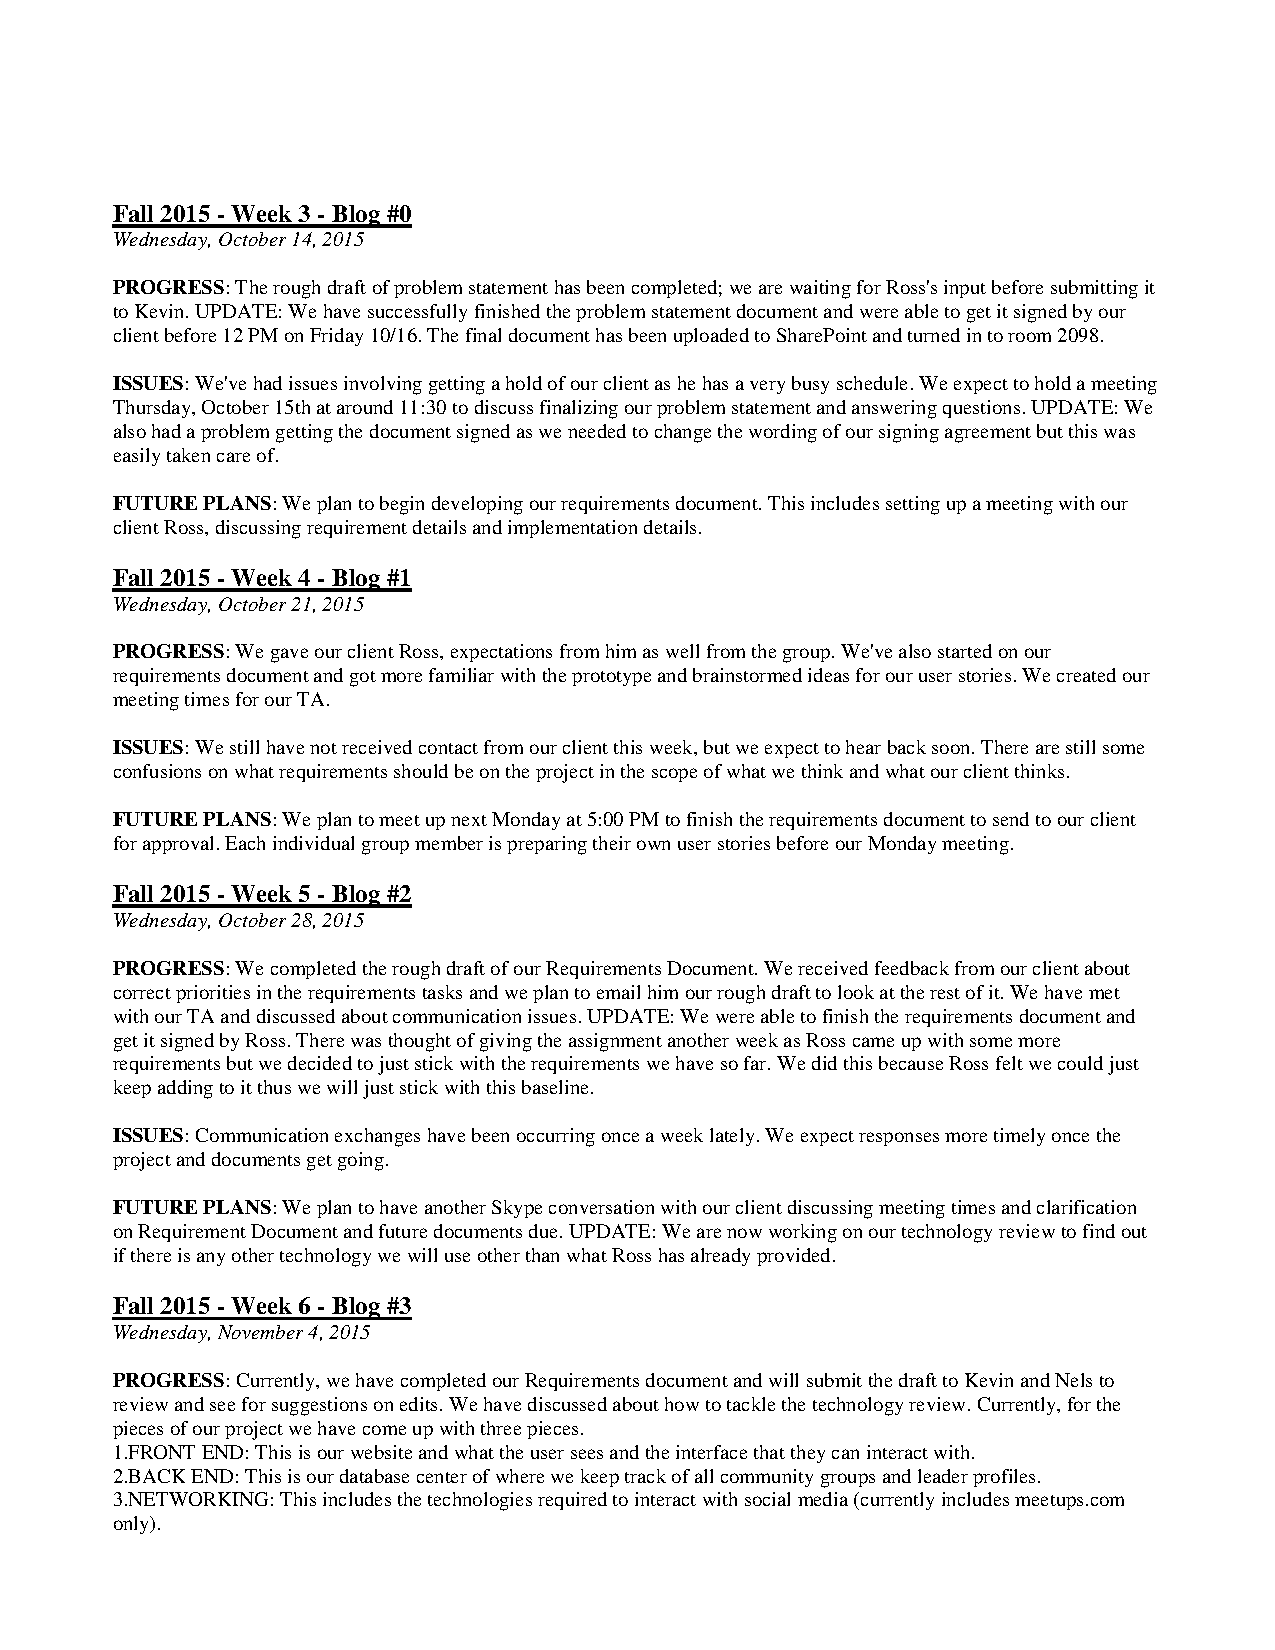
\includepdf[pages={1}, pagecommand={\section{BLOG POSTS}}]{Blog_Posts.pdf}
\includepdf[pages={2-}, pagecommand={}]{Blog_Posts.pdf}


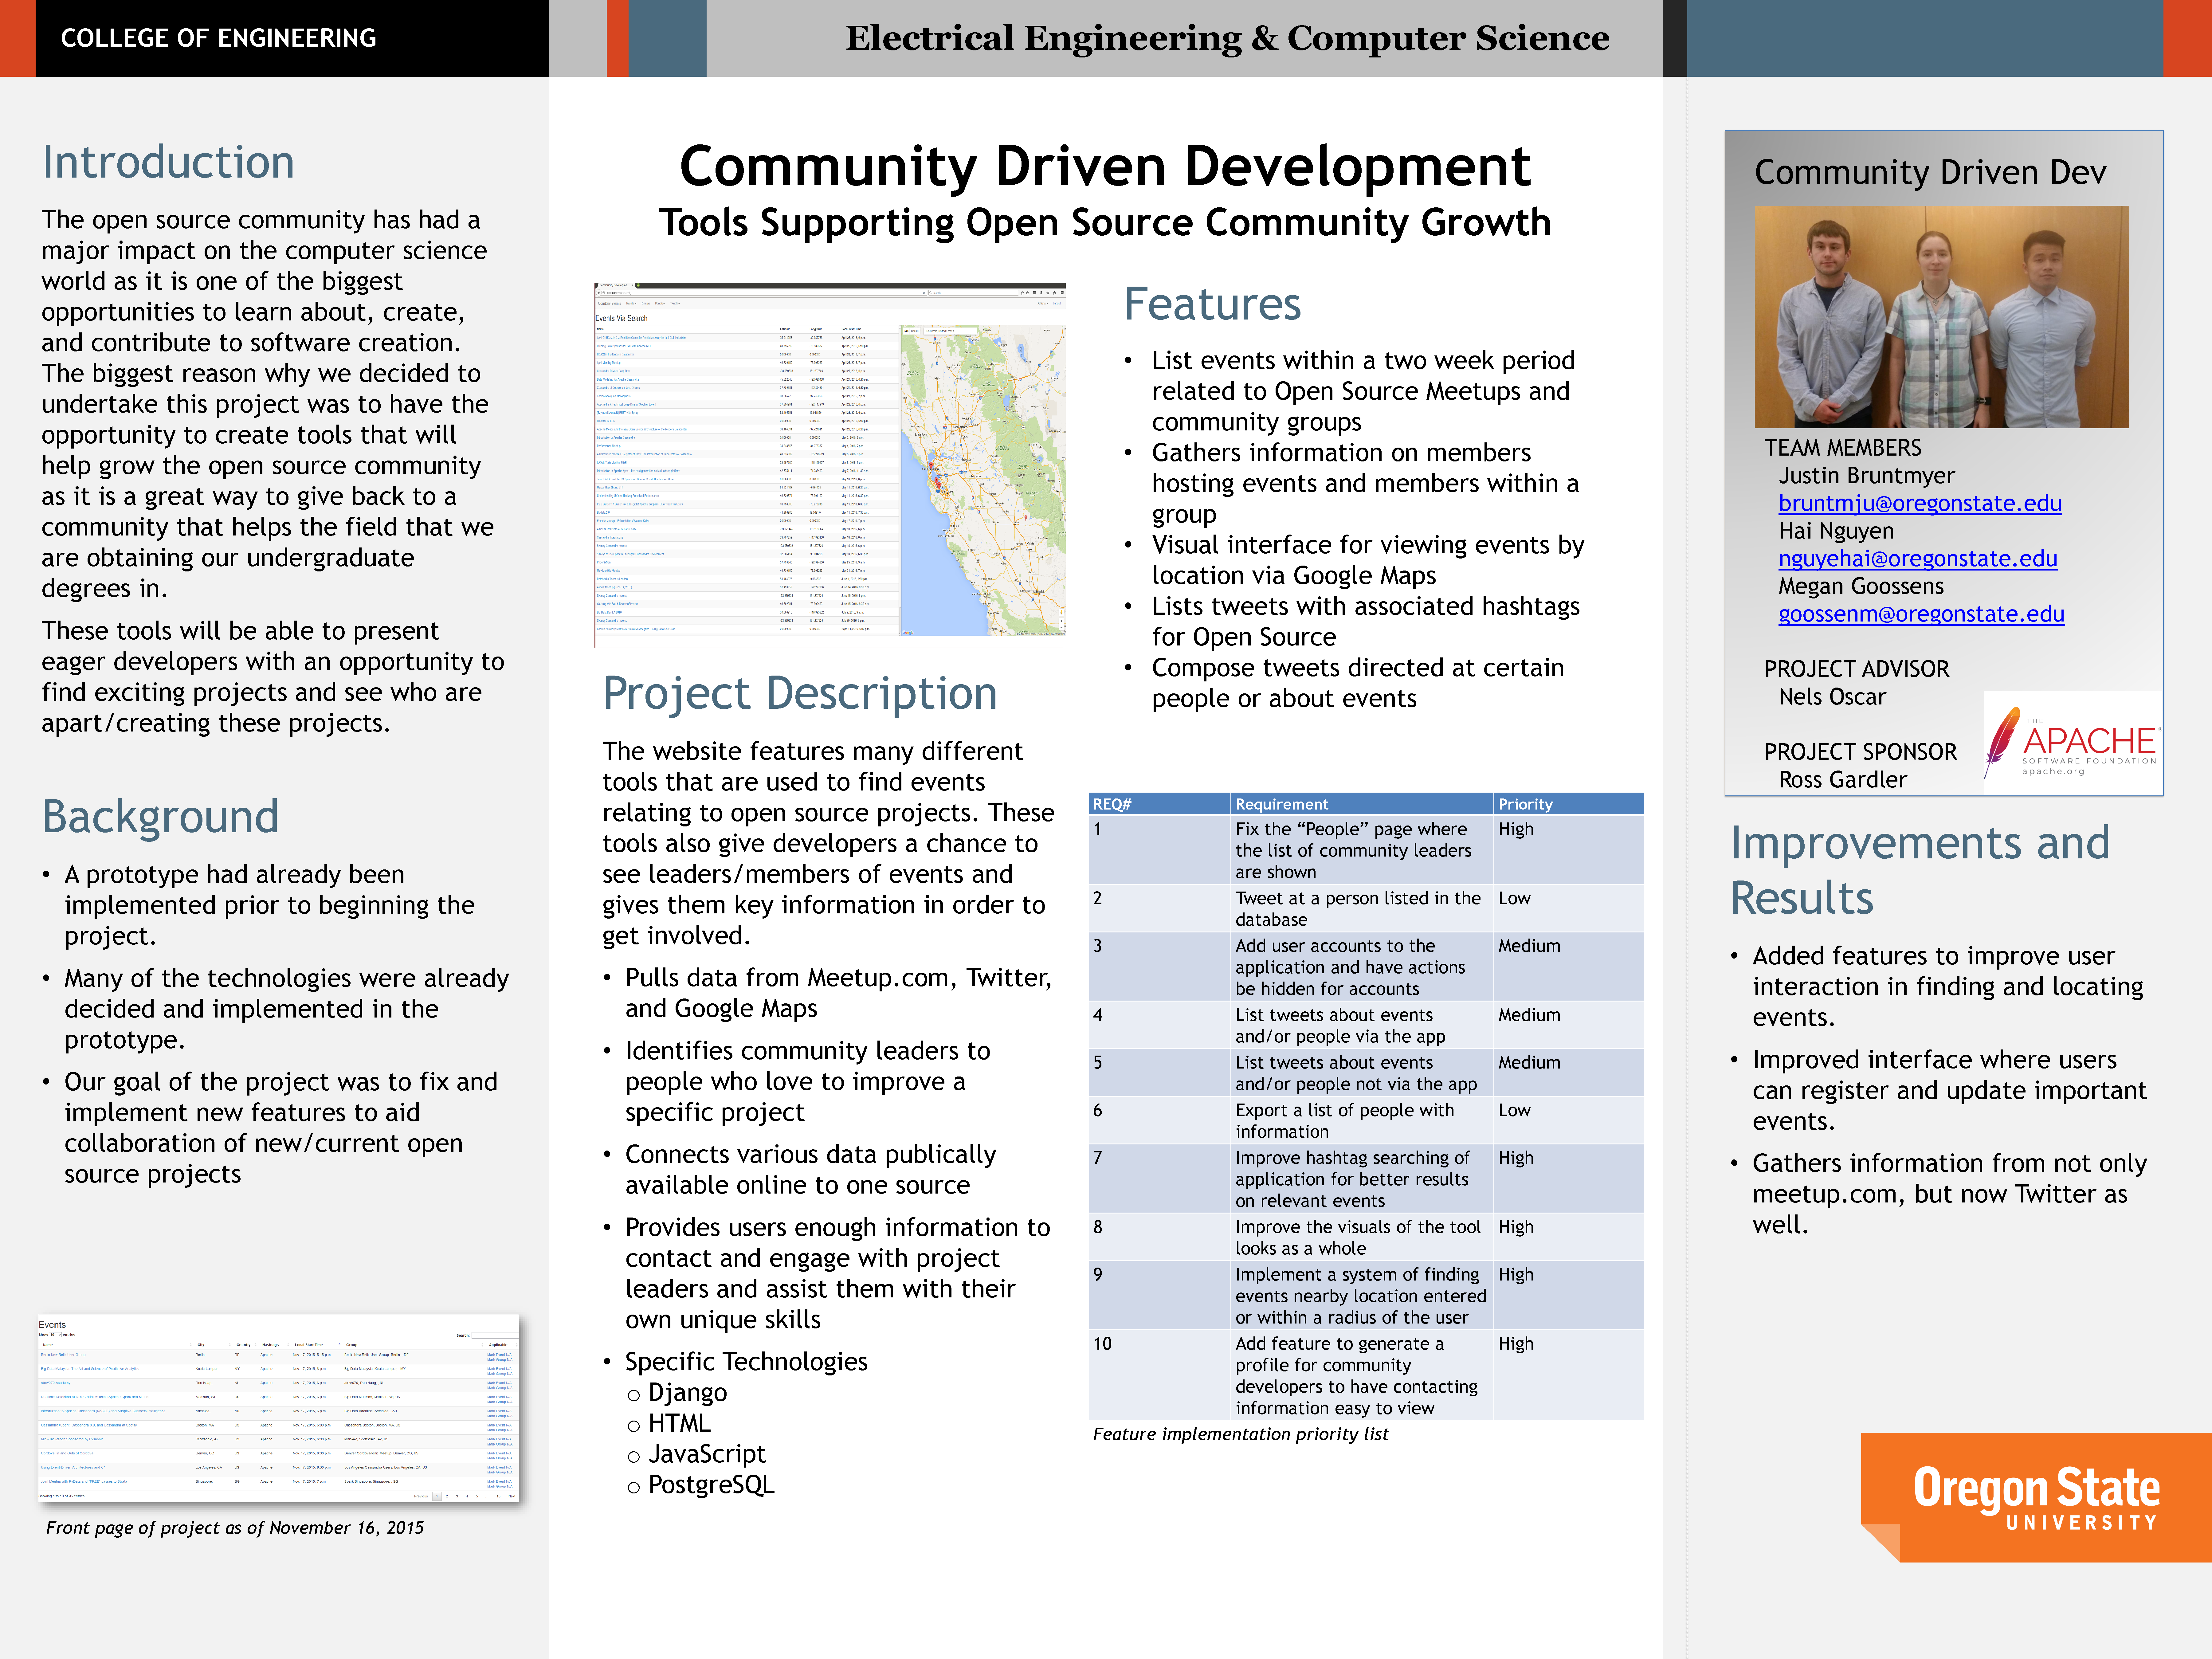
\includepdf[pages={-}, pagecommand={}, angle=90]{poster.pdf}

\section{PROJECT DOCUMENTATION}

\subsection{How The Project Works}
Our project is a website built in Django. It uses Docker to maintain a
consistent environment. The code is structured as a typical Django project. The
most important parts are the views and the templates, and the models. Each view
is either a page on the site, such as the events page, or an action, such as
importing meetups. The models define the database. Each model has associated
fields with it, e.g. the group model has name, city, state, and country fields.\\

\subsubsection{Structure of Project \& Theory of Operation}

The structure and theory of operation go hand to hand with this project because the structure was created based on the theory of how this application operates. Below we will be talking about the structure of the project and how that structure is suppose to operate within the application. All the of the main structures of the application will be put together in a flow diagram to illustrate how the structure operates.\\

The structure for the project is simple. The Django framework creates a database using the PostgreSQL database model. From here we 
can create tables within the database which are also known as models. These models are used as sections of the database where we can 
store information in a way that makes sense. The Django framework also sets up an admin interface so that we have complete control
over what happens to the framework. Once the appropriate models are created then there are the pages of where the events, people imported, event hosts, event search by area, view tweets, and logging in will be displayed. Once the pages are set with the HTML we then pull in the information needed to populate those pages.\\

In order to pull the appropriate information the project uses a hashtag search algorithm that takes a list of hashtags inserted into the database and queries meetup.com with an API call for meetup's that match the hashtags that we have stored. The API call returns the meetup information in the form of Json. The application then parses the Json information returned by the API call searching specifically for the information that we requested such as longitude, latitude of meetup, start time, who hosts the event, country, state, address, event name, group hosting, picture, and source page address for the meetup. All this information is stored in the database under the appropriate model and then pushed the HTML page where the HTML can access and display this information to the user. \\

Now that events have been pulled in we can pull the information for the people associated with a group and hosts of events. To import the people within a certain group the application takes the group ID and make an API call to meetup.com to give the information of who is in that group. The information is returned to the application in a Json format, the data is parsed and is stored in the database under the appropriate model with information such as twitter handle, address, longitude, latitude, name, picture, topics, meetup ID, and last activity. The information is then stored in the database and then can be accessed by the HTML pages to be displayed to the user. To import the event hosts the application take the events hosts ID's that have imported along with the events and then created an API call to meetup.com that asks for information for every event host ID that has been imported. The information is returned in Json format and parsed then stored in the database. The associated pages then have access to the database using HTML to be displayed to the user. \\

Once all of the information has been imported a user can export information about people or events using the export button at the top of the associated page for events and people. The exported lists includes biography information, twitter handles, start times, etc. that is information pertinent for the events or for the people. The login structure is also run by the Django framework with the Django authentication system which keeps track of the usernames and passwords created. The authentication checks the database with the credentials submitted at login and allows the user to login or be denied. Once a user has logged in they have full access to importing functions or marking groups as not applicable. \\

All of the technology that operates for this project is happening in a docker container. A docker container's wrap up a piece of software in a complete filesystem that contains everything it needs to run: code, runtime, system tools, system libraries – anything you can install on a server. This guarantees that it will always run the same, regardless of the environment it is running in. The docker container wraps up our Django application so that it can be run on a local machine in order to be developed on. This is also how the application can be hosted on a web server. Our client and the team that worked on this before us found this to be the best way to run the application for development purposes. The docker container is running as a service on the local machine to open the local host to hosting the application.

The structure of the project can be shown in the diagram below:



\subsection{How to Install \& Run Application}

The way our team developed on the project was using the docker container for Linux as we had countless troubles getting the container to run on the Windows platform. For the purposes of giving the best information on how to install and start this application on a local machine we are going to go over the installation process of what we know to work. Thus, below is a step by step installation process for getting the docker container to run correctly on a Linux operating system and starting the application. \\

\begin{enumerate}
	\item Install and Run Docker for Linux \\
	Docker requires a 64-bit installation regardless of your Ubuntu version. Additionally, your kernel must be 3.10 at minimum. 
	The latest 3.10 minor version or a newer maintained version are also acceptable. Kernels older than 3.10 lack some of the 
	features required to run Docker containers. These older versions are known to have bugs which cause data loss and frequently 
	panic under certain conditions.\\
	
	To check your current kernel version, open a terminal and use uname -r to display your kernel version:
	
	\begin{itemize}
		\item uname -r \\
	\end{itemize}
	
	Log into your machine as a user with sudo or root privileges and open a terminal. Install docker with the command shown below:
	
	\begin{itemize}
		\item sudo apt-get install docker-engine \\
	\end{itemize}
	
	Start the docker daemon with the below command:
	
	\begin{itemize}
		\item sudo service docker start \\
	\end{itemize}
	
	Verify docker is installed correctly with the command below, this command downloads a test image and runs it in a container. 
	When the container runs, it prints an informational message. Then, it exits.:
	
	\begin{itemize}
		\item sudo docker run hello-world \\
	\end{itemize}
	
	You can find more specifics and deal with issues you may encounter here: \\
	https://docs.docker.com/engine/installation/linux/ubuntulinux/ \\
	
	\item Install Docker Machine for Linux \\
	To install docker machine for Linux, run the command below:
	
	\begin{itemize}
		\item curl -L https://github.com/docker/machine/releases/download/v0.7.0/docker-machine -`uname -s`-`uname -m` 
		$>$ \\ /usr/local/bin/docker-machine \&\& chmod +x /usr/local/bin/docker-machine \\
	\end{itemize}
	
	To check if the installation was successful run this command:
	
	\begin{itemize}
		\item docker-machine version \\
	\end{itemize}
	
	\item Installing Django (Python should already be in Linux) \\
	
	To install Django enter these commands into the terminal:
	
	\begin{itemize}
		\item sudo apt-get update
		\item sudo apt-get install python-django \\
	\end{itemize}
	
	\item Download Git Repository from GitHub \\
	
	Open a terminal in a location that you want to store these files. Then enter the commands below to download and switch to 
	appropriate branch:
	
	\begin{itemize}
		\item git clone https://github.com/MaraJade/seniorproject.git
		\item git checkout alpha \\
	\end{itemize}
	
	\item Change Directory and Start Script \\
	
	First you will need to change to the right directory for starting the script. Enter the command below:
	
	\begin{itemize}
		\item cd seniorproject/tools/ \\
	\end{itemize}
	
	From here you run the below command to start the application:
	
	\begin{itemize}
		\item ./scripts/deploy.sh \\
	\end{itemize}
	
	Now you answer the next few questions with these responses in order:
	
	\begin{itemize}
		\item local
		\item Yes
		\item username: (anything you would like)
		\item password: (anything you would like) \\
	\end{itemize}
	
	Now you can go to a web browser and type in the address 0.0.0.0 for your local host and connect to the application. 
	The account you can use right away is the one you just made above. Or you can create a new account. \\
	
	
\end{enumerate}

\section{HOW DID YOU LEARN THE NEW TECHNOLOGY?}

Throughout the project the main technologies that were new to us that we needed to learn were Twitter \& Meetup \& Google Maps API
calls and how they worked, JavaScript, Django, and Docker Containers. With all of these technologies there was a learning curve 
for each of us throughout the project however the most difficult time would have to be during winter term of the project. Winter 
term was the time for us to began development for an Alpha and Beta release. It took some time but we will discuss how we 
learned about each of the technologies and learned how to use them effectively. \\

To learn the API technology for meetup.com, Twitter, and Google Maps there was a lot of documentation deciphering throughout 
the project. We quickly learned that some API's had better documentation than others. The meetup.com API documentation was the 
best of the three because all of the API calls were laid out with a description and examples of what you could do with them. 
There was also a console testing feature on their website that let you test out an API call to see what the result would be 
before you actually use your token to do so. The Google Maps API documentation was decent but still difficult to understand 
in some places as all the technical information of what is happening behind the scenes are not mentioned in the documentation. 
With patience and trial \& error we were able to fully understand what the API was doing and how we could integrate that 
with our displaying of the events on the map plus the search functionality. The last API is also the most difficult to 
understand which is the Twitter API. The documentation did not seem to flow in a way that we could understand clearly. Megan 
began looking at the documentation first and asked for help on the explanation of what was happening and all of us were 
struggling. After taking each section and breaking down what was happening we began to understand the Twitter API more but 
we feel that this kind of documentation should be easier to understand. \\

The next technology that we learned was JavaScript. The main way we all went about learning how to code in JavaScript was by 
practice. The way we would begin to implement items for our requirements were to break down the requirement into sub-tasks and 
then write JavaScript to accomplish those tasks and put them together. The main source of documentation we would use was 
Stack Overflow examples that people have used JavaScript for along with tutorials at W3Schools which is a website with a lot of 
useful tutorials. \\

Django was new to the entire team thus we did a lot of research on the technology in the first couple of months while we were 
creating our documents in the fall. With Django and Python going hand and hand we had an advantage in understanding how to 
make changes in Django. The biggest item we needed to learn was how the framework is working and how the database interacts 
with the application itself. In order to do this we continued to read documentation on Django in order to progress in understanding
it which let to us feeling fairly confident on using Django in the end. \\

The last technology that we had to learn was the docker container and how to run the container. This was a struggle at first as 
we wanted to use the Windows platform to run the application however there were many library complications that we could not 
resolve. Instead we began looking into the docker container and how it runs in a Linux environment. The documentation that we 
found led us to believe that running the container would be a simple process on Linux thus we tried just that. We followed 
the installation guide from the Docker website and had the container running our application fairly quickly. We learned about 
docker machine and running the docker service for Linux through the Docker documentation which was easy to understand. \\

We continued to learn as a team and were willing to help one another whenever we got stuck on a topic. The learning process 
took a huge team effort and contributed to us finishing this project. \\



\section{WHAT DID YOU LEARN FROM ALL OF US? (Justin Bruntmyer)}

\subsection{What technical information did you learn?}
Throughout this project I had the opportunity to learn interesting technical information. The technical information I learned 
a lot about was interacting with API's of several different websites. This not only taught me how to interact with the API
calls and parce the information but it also taught me to read technical documentation for those API's. This was sometimes
frustrating as some websites wrote documentation better than others. Another technical piece of information I learned would
be how to functionally control Django and create an web application from it. I also learned how to manipulate database fields
by parsing information and storing that information within models. \\

JavaScript was also a large portion of technical information I learned from this project. The Google Maps section of this project
was a section I focused heavily on as it interested me. As I continued to learn not only about the Google Maps API but I also 
learned JavaScript coding as the map was basically JavaScript and forced me to understand technically how JavaScript works. \\

I not only had the chance to learn technical information in computer science topics but I also was able to learn a lot about
the technical side of documentation. I learned that writing professional documents as good as you can the first time will bring
better results when it comes to development. Though it is true that documents may need to change such as the Requirements Document
or the Design Document it is important to create the document the first time to the best of your ability as this saves time
and frustration. \\

\subsection{What non-technical information did you learn?}
When reflecting on the project the non-technical information that I learned was mainly how to interact with a client. I learned
right away that communication was going to be the key to having a successful project. The reason I learned this early on is
because I noticed the biggest problems we were having as a group was when the client and our team were not on the same page
for a certain subject. This led to confusion epically when it came to trying to pick a time for having a weekly meeting. This
also taught me that when you are working with people there are going to be different schedules that you are going to have to 
work with in order to make everyone happy on meeting times. \\

Another non-technical piece of information I learned from this project was valuing collaboration with your team. With group
projects in the past, mainly in a class setting of a couple of weeks, I found that the collaboration wasn't all there between
the members because most people just wanted to get it done with and move on which will get you the grade but doesn't necessarily
give you the experience you could have obtained. With working in this team I found that as soon as we spent a lot of time with
one another we began to gel in our coding methods and work with each other to get requirements done correctly, not just done.
What this collaboration experience ultimately taught me is that working towards the benefit of the group as a whole will lift
the group and bring the best out of one another. This was the best non-technical information I learned because it will help me
realize the value of a team as I continue my computer science career. \\

\subsection{What have you learned about project work?}

What I have learned about project work throughout this experience is that client interaction and constant communication is
very important to make sure that everyone is on the same page. This made weekly meetings a priority that had to be met to 
make sure that everyone was on the same page with the requirements, progress being made, and questions that needed to be
answered. I also learned that honesty and communication within the development team is crucial as well. If someone is struggling
on a certain requirement or on a part of a requirement than it is important to communicate those thoughts with the team as 
it can lead to pushing past the issue when everyone gives a hand. This will reduce the risk of requirements being stuck for
many weeks at a time. This means that honesty about being stuck and not knowing a solution is important even if you feel that
it is non-trivial and you should figure it out. \\

I also learned that it is important to \\

\subsection{What have you learned about project management?}

\subsection{What have you learned about working in teams?}

\subsection{If you could have done it all over, what would you do differently?}


\section{WHAT DID YOU LEARN FROM ALL OF US? (Megan Goossens)}
I learned quite a bit from this project. On the technical side, I learned a lot
about interfacing with APIs, and how documentation can either make them easy to
use, or an absolute pain to use. On the non-technical side, I learned about
writing even better reports, as well as how to explain our project in ways that
make it easy for people outside the open source community to understand.  In
project management I learned things like how frustrating it can be when your
client is hard to contact. If I had to do it all over again, I would work harder
to understand exactly what this project is about. We spent a lot of time trying
to understand what our client wanted from each requirement, time that would have
been better spent fulfilling them.

\section{WHAT DID YOU LEARN FROM ALL OF US? (Hai Nguyen)}

\subsection{What technical information did you learn?}
While working on the project, there were many technical concepts that challenged
me that I was mostly unfamiliar with. Since the beginning, I was only
semi-familiar with the concepts of databases, while only working with Python and
MySQL a limited amount of times. For the rest of the technologies from the
project, I learned everything else from scratch. Those technologies include
learning Django, Docker, and API calls. 

With Django, the learning curve for me was gradual. Originally I attempted to
hardcode everything in Python without using the useful tools that Django
provides and adding objects and fields were very difficult. Our client was very
helpful in providing useful documentation that aided us in making our changes
and commits and eventually, Django became second-hand whenever we pushed
changes. 

Docker was mostly hard to handle in the beginning of the project when Justin and
I had difficulty setting up the project on our Windows operating system. After
several days of difficulty without successfully setting up the Docker, we
eventually switched from our Windows system, to developing on a Virtual Machine
with Linux. This made development overall a lot easier with the tools that Linux
provided and all three of the group members on the same operating system.

Lastly, during the development process, the most prominent issue throughout the
three terms were API calls and getting used to all different API’s that we
handled from meetups.com, Twitter, and Google Maps. Since we were handling
different APIs at the same time, keeping track of all and getting used to all
three were particularly difficult when trying to pull the data into our
database.

\subsection{What non-technical information did you learn?}
There are many non-technical aspects that fall under an engineering project. In
terms of the developing process for the project, it was very clear of all of the
documentation that we had to write, that we were accountable for all
requirements that we proposed to do. The project as a whole was scaled to the
perception that we would be working on it throughout the school year for a
couple of hours a week, so we knew in terms of organization, that we needed to
project the amount of work that was reachable for us. 

Specifically for some requirements, we have a development and debug process
where we would develop for a certain feature, but would have to review its
functionality and importance in terms of how much priority that we had to spend
in order to complete the feature and how much time and effort should be spent on
a specific task compared to the entire project as a whole. In terms of a
non-technical aspect, managing our priorities and the process of handling new
feature requests were the most important aspects that we learned.

\subsection{What have you learned about project work?}
Client interaction was prominent where we would get feature requests after some
completed requirements that would satisfy our sponsor. There would be a cycle in
our development process where once we’ve completed a requirements, then our
client would offer feedback and suggestions on the next step or how to take the
feature even further. Most of the time during our development schedule, we did
not account for any stretch goals, but we were able to complete some along the
way.

I learned that preplanning for a project almost rarely goes according to plan or
the schedule. This is especially relevant when we did not understand completely
some requirements that we were given or suggested. It made things very hard to
interpret when some of the requests were over email and we were not able to talk
with our client on a weekly basis; therefore, there was a lot of extrapolation
and interpretation for some of the requests which resulted in some features that
were not in the same intention but ended up satisfying the same needs.

\subsection{What have you learned about project management?}
In terms of project management, while I did not take the main leadership role in this group project, I believe that I did contribute in a way that required leadership and management that was successful for our performance as a whole. Originally, my role in the group became the scribe and pinpointed issues in some particular efforts in the code. Eventually, as the term progressed, we diverged as a group into similar roles for everyone because each of the group members carried over the same amount of responsibility from each other.

Specifically, there are some aspects of project management that I learned that will carry over to my career and other projects. The most important aspect and knowing the responsibilities of each group member and their task to complete the issue. On plenty of occasions throughout the terms, our group as a whole had deadlines to complete with specific tasks designated for each group member. Although it was not anyone's job specifically to keep others in check, it still became important that as a group, we were consistently progressing to reach our goal to complete each requirement.

\subsection{What have you learned about working in teams?}
In the real world, especially in the Computer Science field, it will be very rare to start and complete projects that require individual work. On many if not all occasions, projects will be completed in groups ranging from 5 to thousands of different programmers at once. This is due to the aspect of so many features that go into a single program and all checks and debugging that needs to be done. This project is no exception. Even at our development stage, it is an open source project, which means that we as a group are not the only individuals working on the project, but rather, we are contributing to the Apache Software Foundation as a whole.

\subsection{If you could have done it all over, what would you do differently?}


\section{PROBLEMS ENCOUNTERED}

Throughout this term we have encountered many problems that have impeded our
progress for this project. This was to be expected as with all projects.  Events
occur that can halt progress and bring forth challenges that, as a group, we
needed to overcome. The problems that we have faced are listed below along with
the methods we used to get through the situation. We also ran into the occasioin
coding block where we would have days where not much progress was obtained.
However, we feel this did not impeded our progress as it is just part of being a
computer scientist.

\subsection{Problem 1}
Deciding which platform we were going to be developing on using Docker. This was
a major issue as we originally planed to work with the Windows operating system
however we could not get the application to run locally on a Windows platform.
We continually ran into errors with creating a local database along with having
the right Docker tools to support the application. We had available resources
such as a README file that gave insight on the problem but whatever we tried did
not seem to work. We eventually shifted gears and decided to try Docker and the
application on Linux, specifically Ubuntu 14.04. Thanks to the Linux knowledge
of Megan Goossens and plenty of online documentation we were able to get Docker
installed successfully along with running the application on a local host. From
this point we decided to continue developing in the Linux environment.

\subsection{Problem 2}
At the end of the Fall 2015 term we set up a weekly meeting with our client
throughout Winter 2016 to discuss implementation details for the week and
planned to utilize this time to make sure everyone is on the same page. Due to
some miss-communication we were unable to meet with our client for the first two
weeks. This halted our progress with because we had a lot of issues with getting
Docker to work with Windows and we were counting on a meeting with our client to
resolves those issues as soon as possible. We eventually got in contact with our
client and figured out what was happening as the first week our client was on an
unexpected trip to the UK and in the second week our client did not realize that
these meetings occurred every week throughout the term. These things happen and
once we all had a chance to get on the same page every weekly meeting is going
smoothly. This problem also happened at the beginning of the spring term. A new
weekly meeting time was set up with our client however our client believed that
our first meeting was in the middle of June. This was a problem as we tried to
set up a new meeting time but our client was very busy with travel and vacation
that we were not able to meet with him three weeks prior to expo. Email communication
was very difficult as well.

\subsection{Problem 3}
During week three of Winter 2016 we ran into the issue of meetings being
cancelled due to illness and injury. One of our team members experience an injury
that caused a full group meeting with a TA to occur which halted our progress in
having to get everyone caught up on the same page. This same week another group
member became sick and could not make it to two meetings for the week which
meant that two people could not make it so two meetings were cancelled out of the
weekly three meetings we have as a group. However, we were
able to work individually at home but it was still a noticeable disruption from
the normal work we produce in a week. It did not seem like it was going to
effect the group at first however when we began to get back on track it took
some adjustments to makes sure everyone was on the same page and try to make up
for the week we missed.

\subsection{Problem 4}
During the first week of the term we began developing based on the requirements
we had listed in our requirements document. The problem we ran into here was
that we had issues understanding what are requirements were trying to say thus
we went through the document and changed the language used for the requirements.
This did not change the requirement but it made it easier to understand if
someone is reading through it. This took a days worth of progress which was
frustrating due to the fact that we believed to have this done last term. We
currently are happy with the updated requirements document as it has been
approved by our client, professor, and TA. This halted our progress by being an
unnecessary step in the implementation process as it should have been completed
last term.

\end{document}
